\chapter{Combined search for invisibly decaying Higgs bosons in hadronic channels}
\label{chap:higgstoinv}

\initial{P}articles that escape the detector unseen in any experiment make them, by design, notoriously difficult to search for. The Higgs boson is particularly troublesome with its small production rate at the \acrshort{lhc}, and a predicted branching ratio to invisible states to match. As described in Chpt.~\ref{sec:theory_higgs_to_inv}, the leading estimates are still far higher than the \acrlong{sm}'s value. For the best chance of observing this decay, the inclusion of all of the Higgs boson's production modes is a necessity.

%=======
\begin{easylist}[itemize]
    \easylistprops
    & Add a section or subsection somewhere regarding analysis tools. Perhaps add a brief description of \ROOT (and how it's entrenched in HEP even though people are tending to move away from \ROOT-based analysis onto more industry-standard tools), then lead into the FAST tools and using dataframes, vectorisation, etc., with only small interfaces to \ROOT (for I/O) to extract data. Potentially mention how the data tiers work in CMS (RAW, DIGI, RECO, AOD, miniAOD, nanoAOD, etc.)

    & Emphasize my contributions: control region construction and studies, background estimation, ttbar systematics, and other studies I will have conducted by the time I write up (check AN, chip and HToInv-nanoAOD-tools MRs, and git commit history).

    & Maintaining CMS internal analysis note, documenting all aspects of the analysis. I will first add all relevant information there which I can subsequently use when writing this chapter.

    & Since it's my thesis, I can talk about \ttH, \VH and \ggF/monojet, even though the Bristol contribution to the final, public result may only be \ttH and resolved \VH. Would need to be able to run the fit for all three modes simultaneously, ensuring we have complete (and correct) systematics for \ggF.
\end{easylist}

% Can pull from Section 37 of my lab book, and all the talks I and other people from the team have given (Presentations and talks/ folder, also Other peoples/ subdirectory). Can also pull from AN for analysis strategy


%=========================================================


\section{Production modes of the Higgs boson}
\label{sec:htoinv_production_modes}

At the \acrshort{lhc}, the most common mechanisms for producing a Higgs boson are \acrfull{vbf}, gluon-gluon fusion (\ggF), associated production from top quarks (\ttH), and associated production from a vector boson (\VH). Feynman diagrams of these processes are shown in Fig.~\ref{fig:higgs_feynman_diagrams}. They have very different characteristics, production rates, and event signatures, complementing each other and allowing a single analysis to cover all bases with orthogonal parameter spaces to target them individually.

\begin{figure}[htbp]
    \centering
    \begin{subfigure}[b]{0.45\textwidth}
        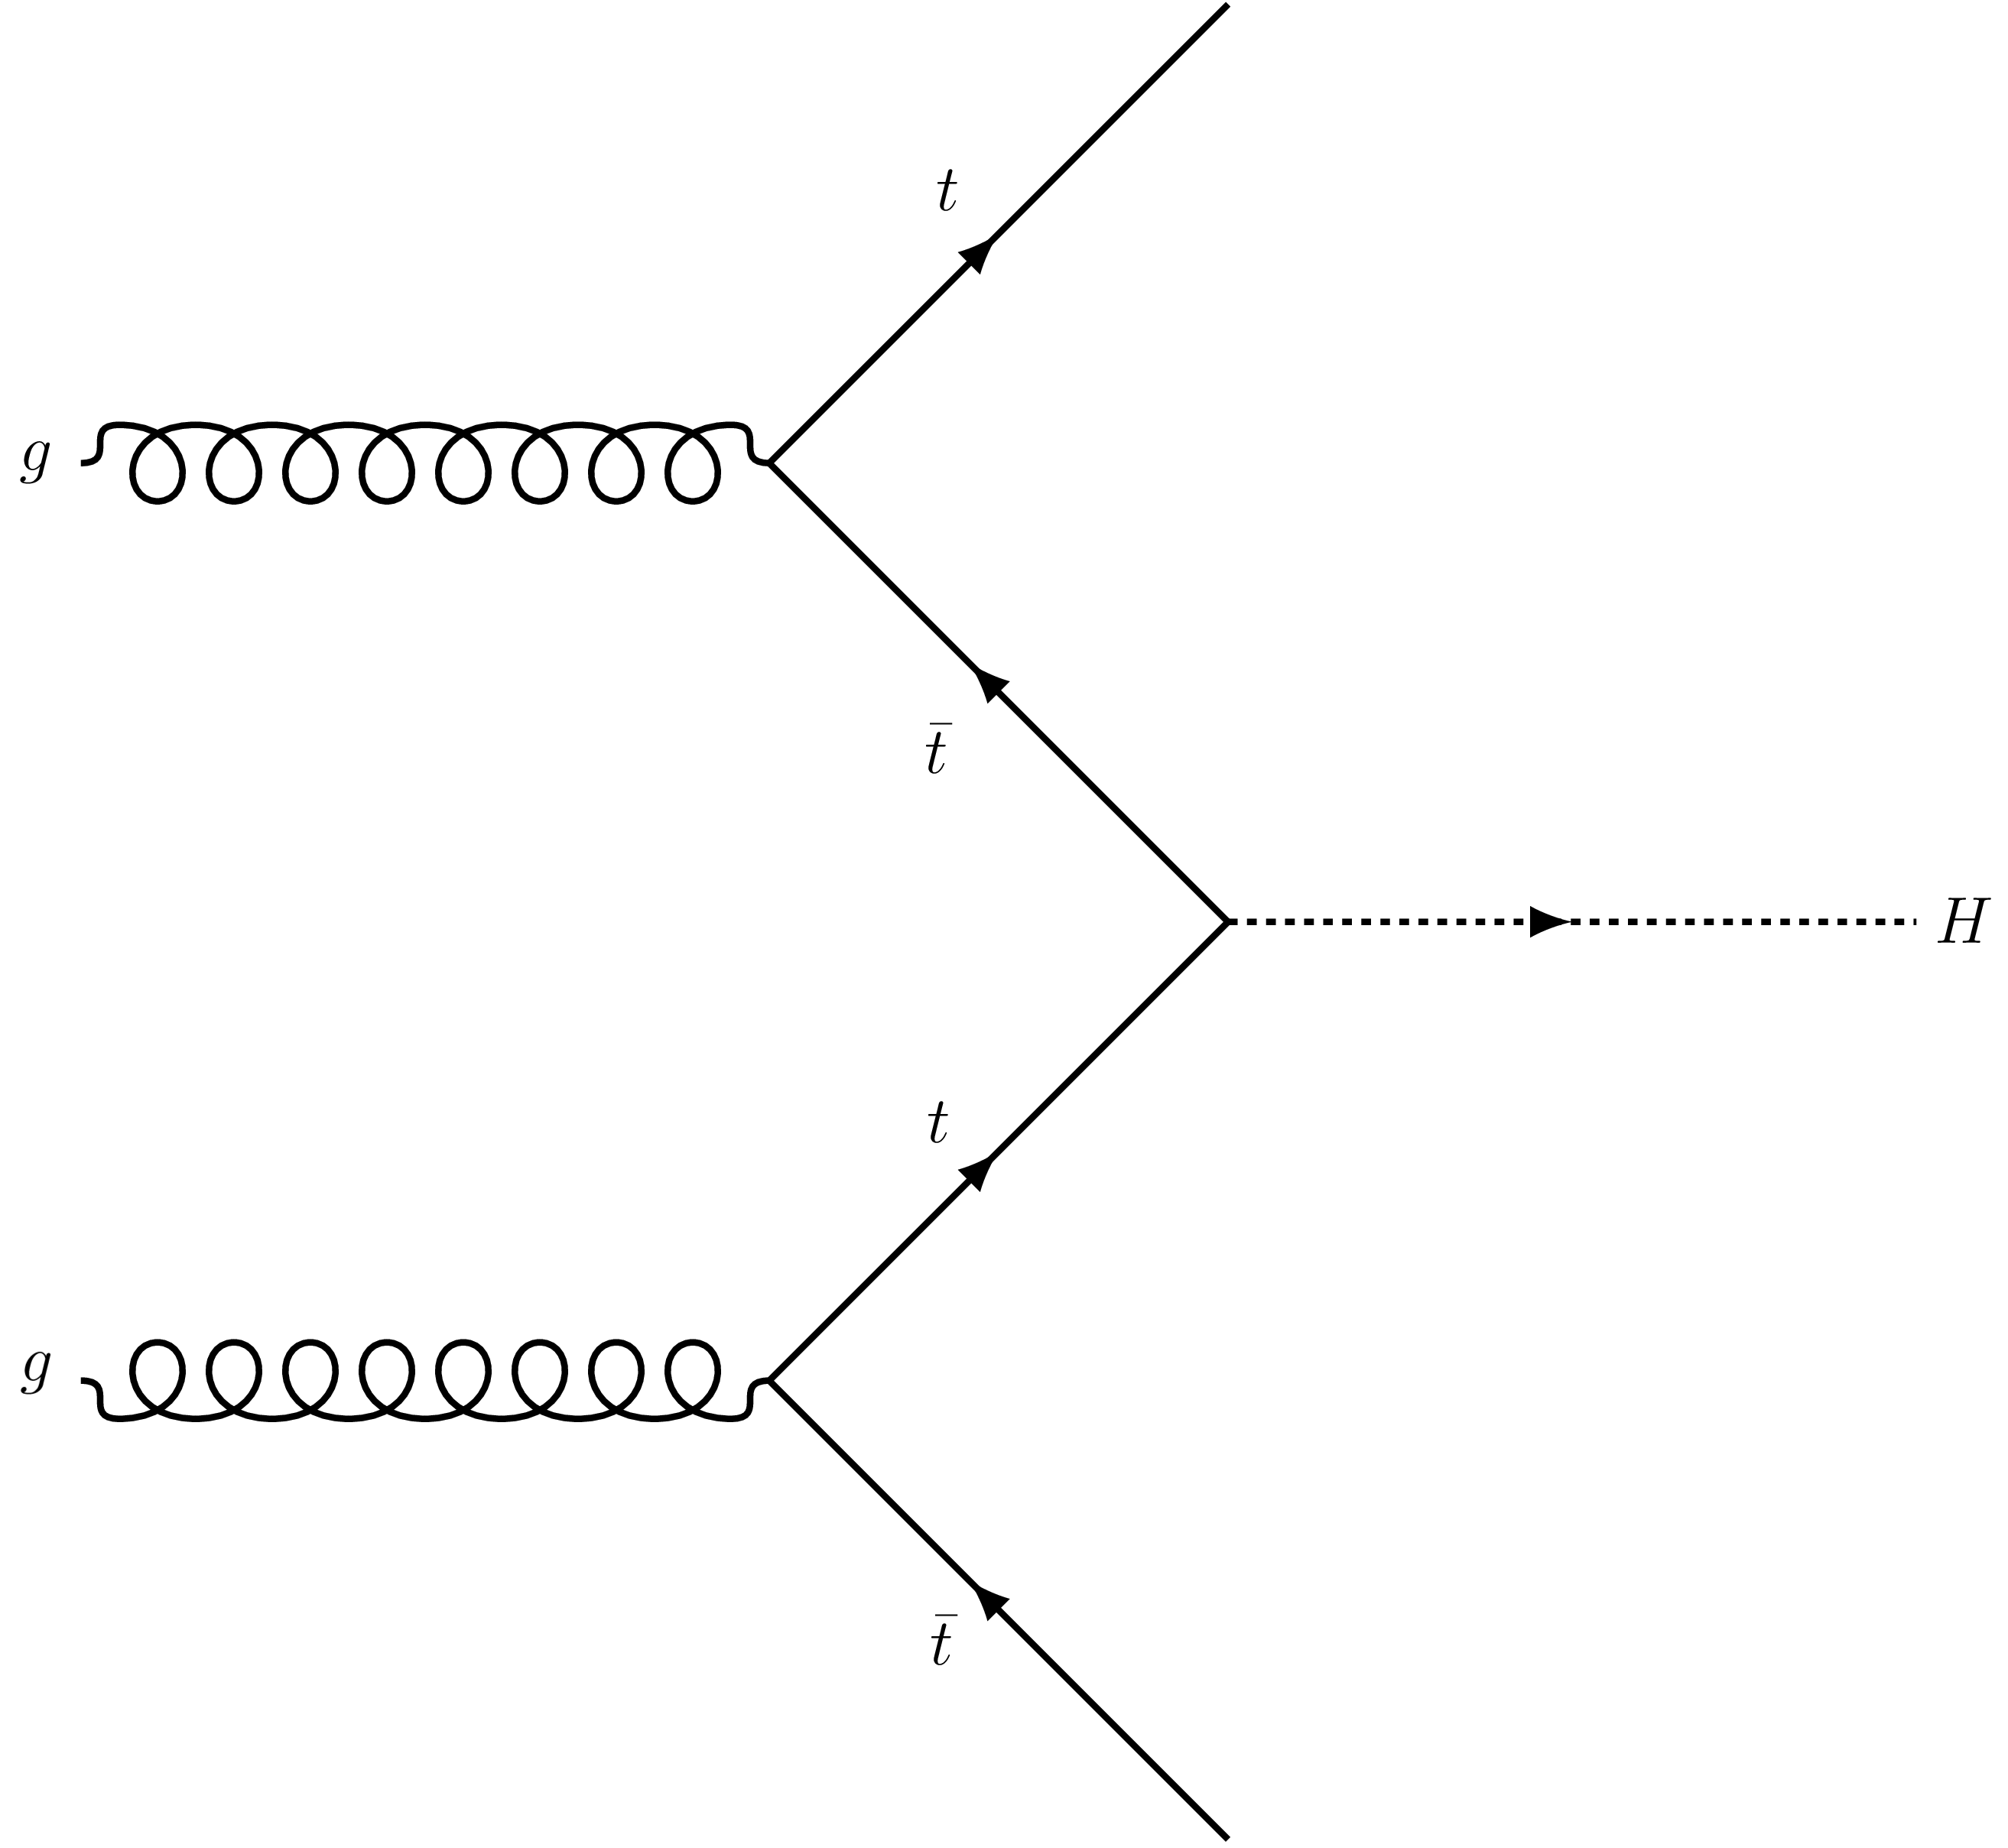
\includegraphics[width=\textwidth]{figures/feynman_diagrams/ttH.png}
        \caption{\ttH}
    \end{subfigure}
    \hfill
    \begin{subfigure}[b]{0.45\textwidth}
        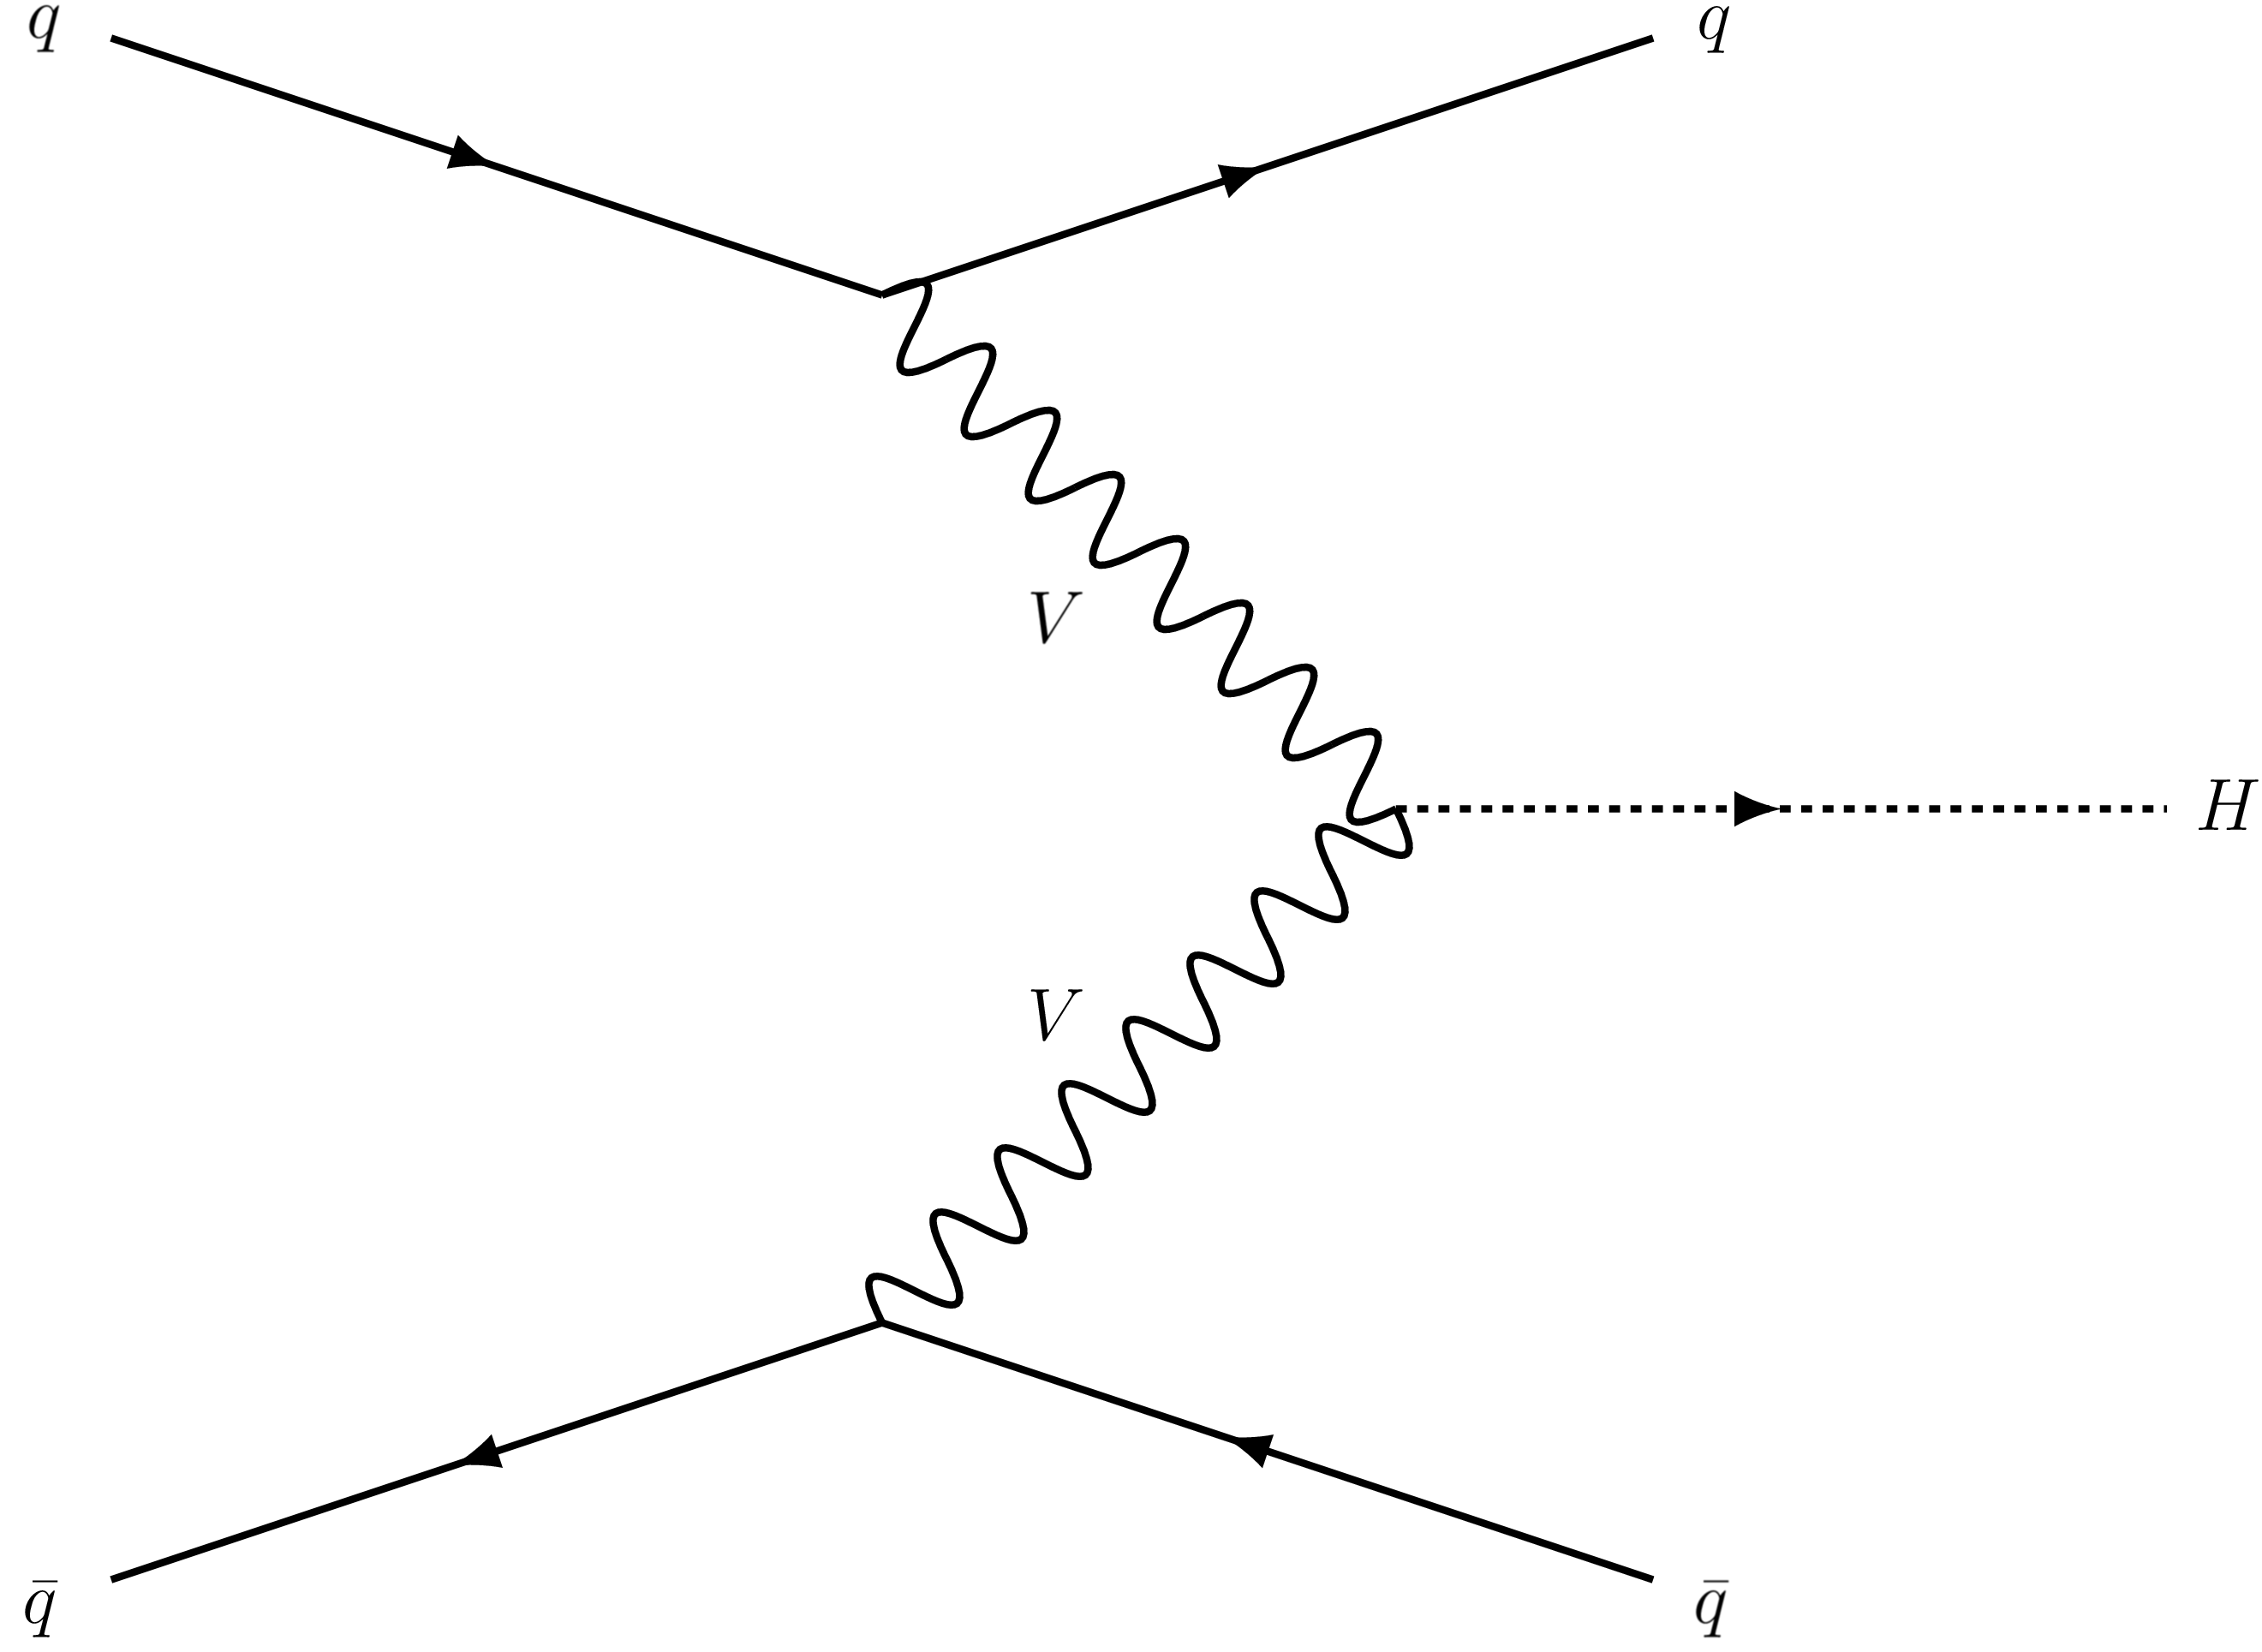
\includegraphics[width=\textwidth]{figures/feynman_diagrams/VBF.png}
        \caption{\acrshort{vbf}}
    \end{subfigure}
% blank line to start new row
    \begin{subfigure}[b]{0.45\textwidth}
        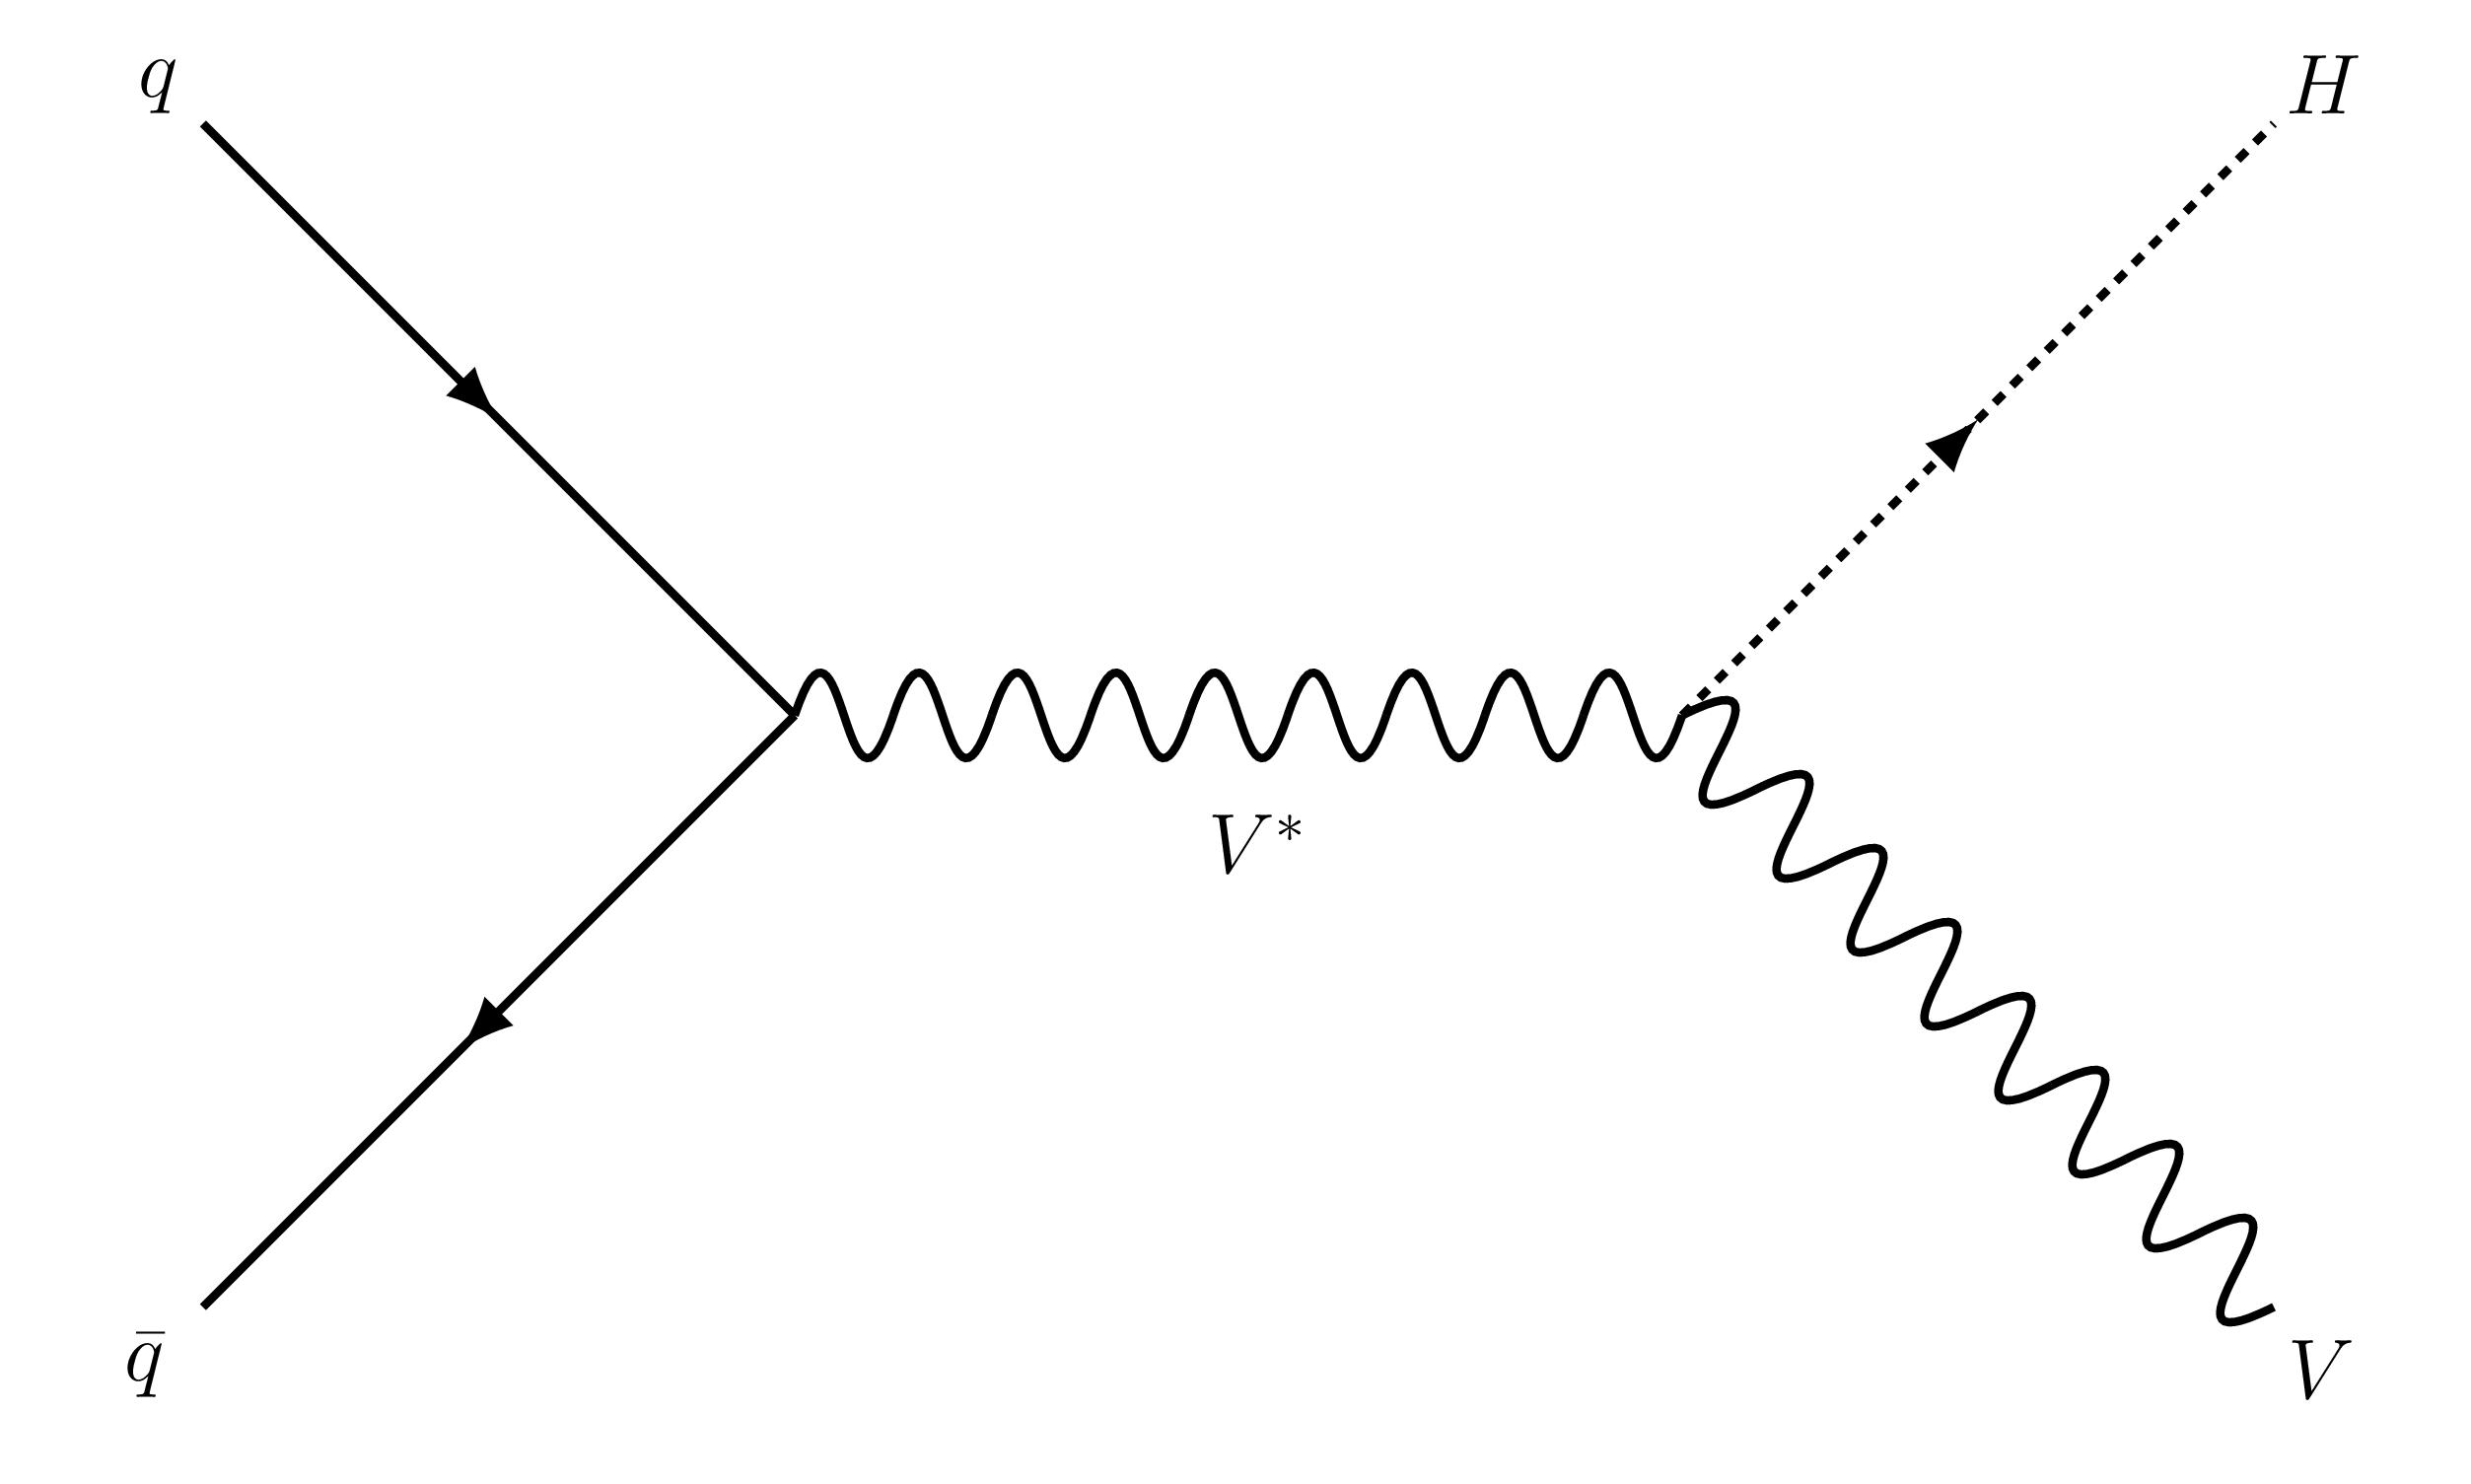
\includegraphics[width=\textwidth]{figures/feynman_diagrams/VH.png}
        \caption{\VH}
    \end{subfigure}
    \hfill
    \begin{subfigure}[b]{0.45\textwidth}
        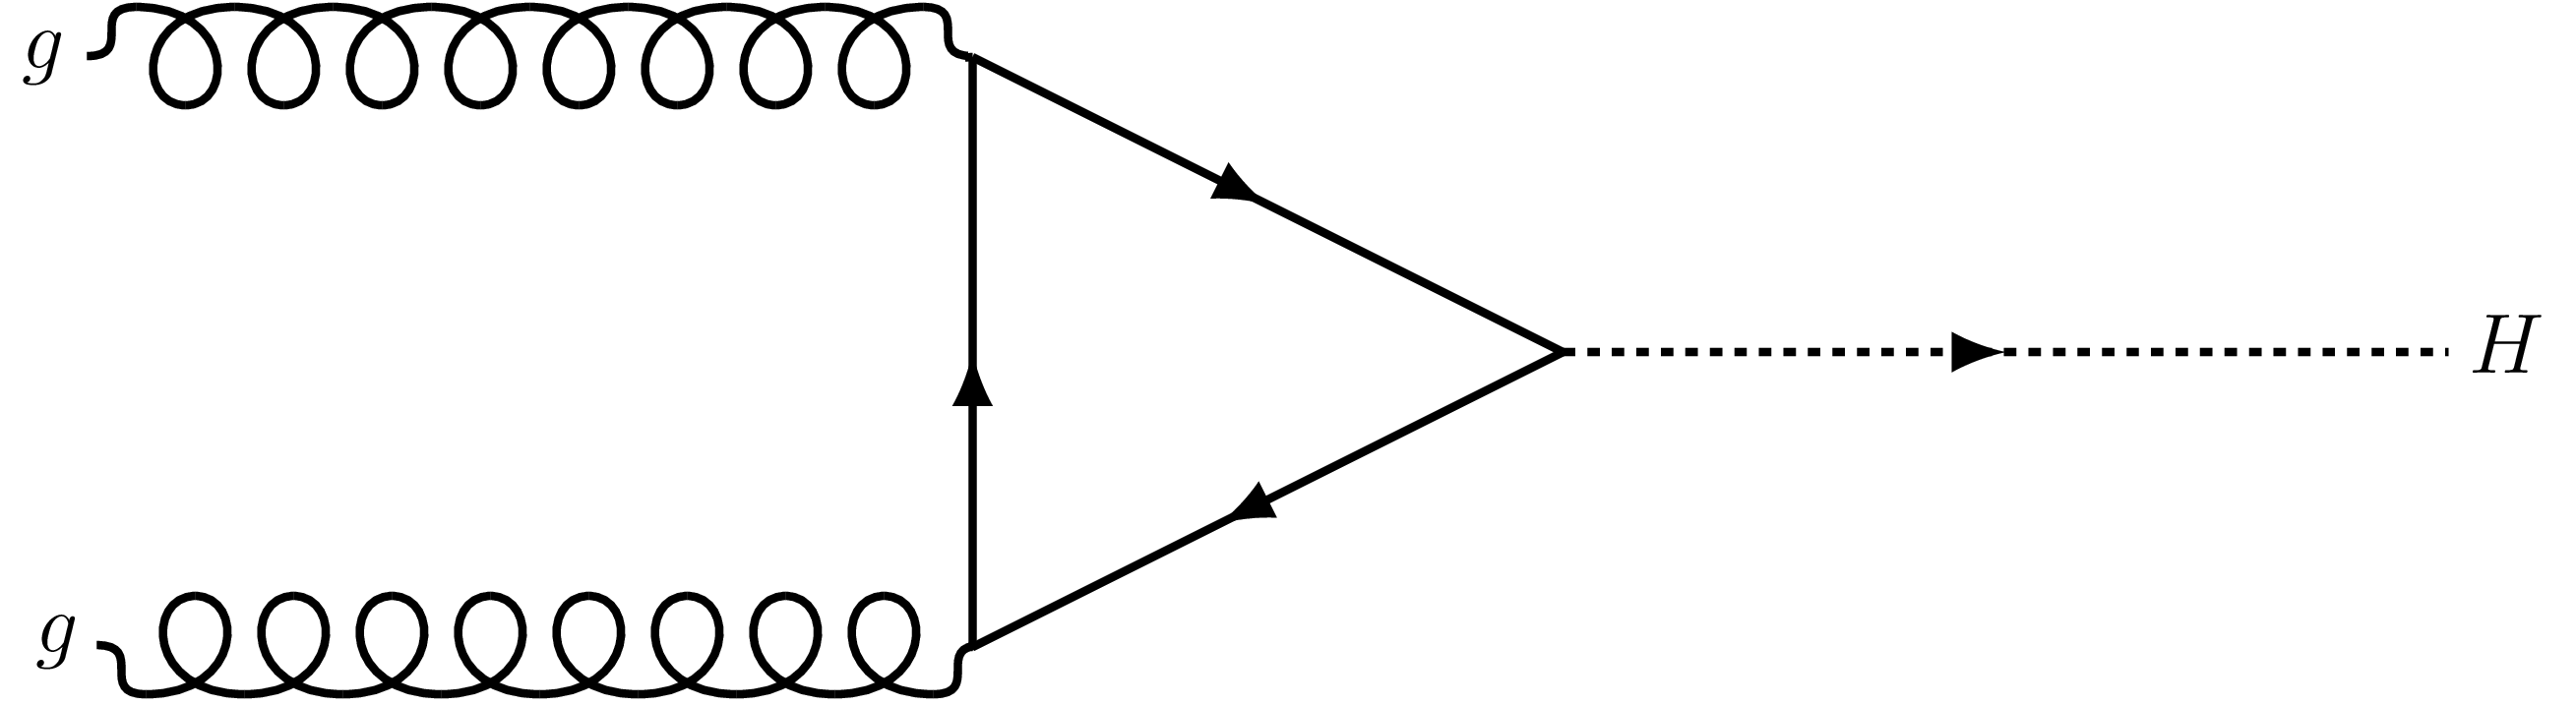
\includegraphics[width=\textwidth]{figures/feynman_diagrams/ggF.png}
        \caption{\ggF}
    \end{subfigure}
\caption[A subset of the Feynman diagrams for the four predominant production mechanisms of the Higgs boson at the LHC]{A subset of the Feynman diagrams for the four predominant production mechanisms of the Higgs boson at the \acrshort{lhc}.}
\label{fig:higgs_feynman_diagrams}
\end{figure}

% Additional diagrams for ggF are a square top loop (gluons join the two vertices on the left), where the Higgs exits at one of the vertices on the right and a gluon exits at the other. For ZH, can also have gg->ZH as well as pp->ZH. Not sure if it's worth showing them or just describing them.


%=========================================================


\subsection{Vector boson fusion (VBF)}
\label{subsec:htoinv_VBF}

A \acrshort{vbf} topology is exhibited by a \tchannel exchange of two vector bosons radiated by the incident quarks, which then combine to form a new particle such as a Higgs boson. Since the masses of the \PW and \PZ bosons are more than half the Higgs mass, it can easily be produced on shell. The recoil of the quarks characterises the visible system: two \glspl{jet} with a large combined invariant mass, usually with a large separation in pseudorapidity but small in azimuthal angle. The \glspl{jet} move in opposite directions, one in $+\eta$ and the other in $-\eta$, but are usually contained in the same horizontal half of the detector.


%=========================================================


\subsection{Associated production from top quarks (\texorpdfstring{\ttH}{ttH})}
\label{subsec:htoinv_ttH}

In \ttH, two \ttbar pairs are produced. A top quark \Ptop from one pair and antiquark \APtop from the other annihilate to produce the Higgs boson. As it decays invisibly, it is the remaining \Ptop and \APtop in the event that lead to three classes of final state. The \Ptop quark decays almost exclusively to $\Pbottom\PWplus$ (and $\HepProcess{\APtop \to \APbottom\PWminus}$)~\cite{PhysRevD.98.030001}. In a resolved system where top quarks possess low to moderate momentum, the multitude of available \Pbottom-tagging algorithms can distinguish the decays of the \Pbottom quark. The products of the \PW boson is the determining factor of the final state. Hadronically-decaying $\PW\text{s}$ ($\HepProcess{\PW \to \Pquark\APquark}$), of course, produce pairs of \glspl{jet}. But they can also decay into a lepton and neutrino. The final states then all have \ptmiss and up to two \glspl{bjet} in common. Several \glspl{jet} may accompany them (the hadronic channel), or fewer \glspl{jet} with a single lepton (the \emph{semi-leptonic} channel), or two leptons (the dileptonic channel). The magnitude and direction of the \ptmiss in the latter two channels may be affected by the neutrinos, depending on their direction and energy.

In a boosted system where the top quarks have significant \pt, it is often difficult to tag \glspl{bjet}, especially if one is searching in the hadronic channel. Recently-developed algorithms can assist in this case by inspecting AK8 \glspl{jet}---objects clustered with the \gls{antikt} using a radius parameter of 0.8 instead of the usual 0.4. The \deepakeight tagger, explained in Chpt.~\ref{subsec:htoinv_deepak8}, is used in the analysis to classify boosted topologies originating from \Ptop quarks as well as \PVec bosons to identify \ttH events.


%=========================================================


\subsection{Associated production from a vector boson (\texorpdfstring{\VH}{VH})}
\label{subsec:htoinv_VH}

A Higgs boson is radiated by the vector boson \PVec in the \VH mechanism. Parallels can be drawn with \ttH as the decay of the \PVec determines the search channel. Resolved and boosted systems are also possible. In the resolved case, a dijet pair with an invariant mass close to that of the parent boson would distinguish the hadronic channel. \Pbottom-taggers can be exploited if the decay is to a \Pbottom quark, i.e., $\HepProcess{\PWplus \to \APbottom\Pquark_{\Pup}}$,\footnote{I'm not sure what the symbol is (if there even is one) for an up-type quark. Maybe $\Pquark_{\Pup, \Pcharm}$ to be more specific, or $\Pquark_{\uparrow}$?} $\HepProcess{\PWminus \to \Pbottom\APquark_{\Pup}}$, or $\HepProcess{\PZ \to \Pbottom\APbottom}$. Single lepton channels are possible for \WH and dilepton for \ZH. For a boosted \PVec, one expects the products to the collimated into a single AK8 \gls{jet}, at least in the hadronic channel. As with \ttH, we take advantage of \deepakeight to capture these scenarios. 


%=========================================================


\subsection{Gluon-gluon fusion (\texorpdfstring{\ggF}{ggF})}
\label{subsec:htoinv_ggF}

Despite \ggF having the largest cross section of the four modes, its upper limit on $\BRof{\higgstoinv}$ is the weakest. The Higgs boson is created through the loop-level fusion of the initial state gluons, normally mediated by a top quark since it has the largest coupling to the Higgs. With no additional final state particles at first order, searches for this production mode usually involve initial state radiation from the gluons or the loop. As such, the signature is at least one \gls{jet} and \ptmiss.


%=========================================================


\section{Results of previous searches}
\label{sec:htoinv_prev_results}

Many previous analyses have investigated the \higgstoinv decay, in some cases from dedicated searches, but often as an afterthought or interpretation of the main analysis. \acrshort{vbf} is the most sensitive production mode. This is demonstrated in Tab.~\ref{tab:hinv_br_limits} by the upper limits attained compared to the other mechanisms. In Ref.~\citenum{Sirunyan:2018owy}, a combination was performed by \acrshort{cms} over all the productions modes detailed in the table (with the exception of \ttH). Using the recent 2016 measurements as well as data taken from Run-1 and 2015, this combined observed upper limit sits at 19\,\%, while the expected is 15\,\%. With only data from Run-1 and 2015 (the previous combination) the observed and expected upper limits of 24\,\% and 23\,\%, respectively, were found~\cite{Khachatryan:2016whc}.

\begin{table}[htbp]
    \centering
    \begin{tabular}{lllcc}
        \hline
        Targeted mode & Analysis & Final state & Observed UL & Expected UL\\\hline
        \acrshort{vbf} & Ref.~\citenum{Sirunyan:2018owy} & $\text{\acrshort{vbf}-\glspl{jet}} + \ptmiss$ & 33\,\% & 25\,\% \\
        $\ZH(\HepProcess{\PZ \to \Plepton\Plepton})$ & Ref.~\citenum{Sirunyan:2017qfc} & $\PZ(\HepProcess{\to \Plepton\Plepton}) + \ptmiss$ & 40\,\% & 42\,\% \\
        $\ttH$ & Ref.~\citenum{CMS-PAS-HIG-18-008} & $\ttbar(\HepProcess{\to \text{\glspl{jet}}/\Plepton/\Plepton\Plepton}) + \ptmiss$ & 46\,\% & 48\,\% \\
        $\VH(\HepProcess{\PVec \to \Pquark\APquark})$ & Ref.~\citenum{Sirunyan:2017jix} & $\PVec(\HepProcess{\to \Pquark\Pquark}) + \ptmiss$ & 50\,\% & 48\,\% \\
        $\ggF$ & Ref.~\citenum{Sirunyan:2017jix} & $\text{\glspl{jet}} + \ptmiss$ & 66\,\% & 59\,\% \\\hline
    \end{tabular}
    \caption[The most recent searches for invisibly decaying Higgs bosons with 2016 data from CMS, and the upper limits on the \higgstoinv branching ratio at 95\,\% confidence level achieved]{The most recent searches for invisibly decaying Higgs bosons with 2016 data from \acrshort{cms}, and the upper limits (UL) on the \higgstoinv branching ratio at 95\,\% confidence level achieved. Only the \acrshort{vbf} analysis is a dedicated search, while the others are interpretations of the results obtained in their respective primary analyses. For the $\ttH$ analysis, the hadronic (\glspl{jet}), semi-leptonic (\Plepton), and dileptonic ($\Plepton\Plepton$) channels were combined.}
    \label{tab:hinv_br_limits}
\end{table}

% Might be nice to add a row with the combined (bar ttH) result with only 2016 data.


%=========================================================


\section{Overview of the analysis}
\label{sec:htoinv_analysis_overview}

The analysis discussed in the remainder of the chapter is a dedicated search for invisibly decaying Higgs bosons in hadronic final states, incorporating all four of the production modes from the outset. In contrast to many of the previous analyses that separately set limits on $\BRof{\higgstoinv}$ by reinterpretation, our approach has many benefits. A simultaneous search for all of the production modes allows us to construct search regions to target each one, building in orthogonality to avoid overlap between them. Data and simulation samples, recipes for corrections and systematic uncertainties, the analysis framework, and results can all be shared to provide a cohesive and consistent environment from which to perform the analysis. As well as streamlining the process of the final combination over each production mechanism, communication when establishing the analysis ensures each can cover as much phase space as possible without the trouble of overlap or contamination.

Direct collaboration amongst several institutes divides up the task appropriately. Researchers at the University of Bristol, including as myself, and LLR (\emph{Laboratoire Leprince-Ringuet, \'{E}cole Polytechnique, Universit\'{e} Paris-Saclay}) focus on \ttH and the resolved \VH modes. Those at Imperial College London, who have a long history with the \acrshort{vbf} search~\cite{Chatrchyan:2014tja,Sirunyan:2018owy}, assume responsibility of this process. Researchers at Boston University---who have previously been involved in \acrshort{bsm} analyses with interpretations in invisibly decaying Higgs bosons~\cite{Khachatryan:2016mdm,Sirunyan:2017jix}---specialize in monojet and mono-\PVec searches. This makes them naturally suited to investigating the boosted aspect of \VH, and \ggF.

Emphasis will be placed on the non-VBF modes, particularly \ttH and resolved \VH, as I had direct involvement in those aspects of the analysis. Before Boston University joined our effort, we also studied the boosted \VH and \ggF mechanisms. Accordingly, they will also be given some attention. Definitions of the physics objects used analysis-wide are discussed in Chpt.~\ref{sec:htoinv_objects}. The data from \acrshort{cms} and from simulation, along with required corrections and systematic uncertainties, are acknowledged in Chpt.~\ref{sec:htoinv_data_sim}. These are followed by the event selection in Chpt.~\ref{sec:htoinv_event_selection}. Definitions of the categorisation of production modes and phase space regions are illustrated in Chpts.~\ref{sec:htoinv_categorisation} and \ref{sec:region_definitions}, respectively. Methods for accurately estimating the background processes in the signal region are delineated in Chpt.~\ref{sec:htoinv_background_est}. The incorporation of these and the aforementioned sections in the statistical treatment are presented in Chpt.~\ref{sec:htoinv_satistical_treatment}, before the results of the analysis in Chpt.~\ref{sec:htoinv_results}.

% Given the \acrshort{lhc} is a \emph{hadron} collider, processes with hadronic channels are the natural choices.\footnote{Or should I say ``most sensitive''?} \Gls{met} from the purely-invisible decay of the Higgs---and hadronic activity from the particles associated with the production mechanism---constitute the [final state], often known as a ``\text{\glspl{jet}} + \ptmiss$'' search.


%=========================================================


\section{Definitions of physics objects and variables}
\label{sec:htoinv_objects}

The physics that occurs at the high energies the \acrshort{lhc} is capable of is not simple. That makes the recording of particles and events overall a non-trivial undertaking. Based on complex hardware and software, research, and the experience of previous experiments, defining physics objects and variables from an analyst's standpoint is thankfully straightforward. The basic [definitions] are already included into the \ROOT files we use, with [additional] selections on top to select the analysis-level objects.

Different working points for the identification of many objects are available from the respective \glspl{pog}, trading inclusivity for purity the tighter the selections are. ``Veto'' and ``loose'' criteria are used to specify the secondary leptons in the dilepton \glspl{CR}, and when vetoing leptons and photons (or applying their corresponding veto weights) in the signal region. The ``medium'' and ``tight'' selections are used to construct the primary objects in the \glspl{CR}. We denote these objects with a subscript corresponding to the working point. The requirements elaborated upon in the subsequent subsections.


%=========================================================


\subsection{Jets}
\label{subsec:htoinv_jet_objs}

In the \nanoAOD data tier, a \gls{jet} is defined as an AK4-clustered, charged hadron-subtracted object reconstructed with the \gls{particleflow}, with \acrlong{jec} applied and a requirement of $\pt > \text{15}\GeV$. For the analysis, we raise the threshold to $\pt > \text{30}\GeV$ and explicitly require $\abseta < 5.0$. Either the tight, or tight $+$ lepton veto, \acrshort{pf} identification requirements are [also] mandatory to establish a sufficient degree of purity with a very high efficiency ($> \text{98\,\%}$ in all $\abseta$ regions). These are documented in Tabs.~\ref{tab:htoinv_jet_id_def_2016}, \ref{tab:htoinv_jet_id_def_2017}, and \ref{tab:htoinv_jet_id_def_2018}. Finally, \glspl{jet} must not overlap (i.e., $\Delta R > \text{0.4}$) with any \vetoEle, \looseMuon, or \loosePhoton in the event to avoid potential misidentification.

AK8 \glspl{jet} follow the same reconstruction and identification prescription as AK4 \glspl{jet}, only differing in the cone size.\footnote{I'm not what/if the minimum \pt of an AK8 \gls{jet} is, and whether they have an $\eta$ restriction (I've seen $\abseta < 2.4$ in a few places, but nothing confirmed).}

A \gls{bjet} is defined as a \nanoAOD \gls{jet} with $\pt > \text{20}\GeV$, $\abseta < 2.5$ (2.4 in 2016), and to satisfy the medium working point (a mis-tag rate of 1\,\%) from the \deepcsv algorithm~\cite{Sirunyan:2017ezt}.

% Might need to say we use pt_nom for all instances of pt thresholds (except noisy EE jets in 2017 where the raw pt is used). pt_nom is created offline and is additionally jet energy resolution-corrected (maybe check nanoAOD-tools for specifics)


%=========================================================


\subsubsection{2016}
\label{subsubsec:htoinv_jet_objs_2016}

The tight and tight $+$ lepton veto ID requirements are detailed in Tab.~\ref{tab:htoinv_jet_id_def_2016}. Specifically to this year, all \glspl{jet} are required to satisfy the criteria for the tight pileup ID to ensure they do not originate from pileup vertices.

\begin{table}[htbp]
    \centering
    \begin{tabular}{lcccc}
        \hline
        Criterion & $\abseta \leq \text{2.4}$ & $\text{2.4} < \abseta \leq \text{2.7}$ & $\text{2.7} < \abseta \leq \text{3.0}$ & $\abseta \geq \text{3.0}$ \\\hline
        Neutral hadron fraction & $< \text{0.90}$ & $< \text{0.90}$ & $< \text{0.98}$ & --- \\
        Neutral EM fraction & $< \text{0.90}$ & $< \text{0.90}$ & $> \text{0.01}$ & $< \text{0.90}$ \\
        \# constituents & $> \text{1}$ & $> \text{1}$ & --- & --- \\
        Muon energy fraction & $< \text{0.80}$* & $< \text{0.80}$* & --- & --- \\
        Charged hadron fraction & $> \text{0}$ & --- & --- & --- \\
        Charged multiplicity & $> \text{0}$ & --- & --- & --- \\
        Charged EM fraction & $< \text{0.99}$ (0.90*) & --- & --- & --- \\
        \# neutral particles & --- & --- & $> \text{2}$ & $\text{10}$ \\\hline
    \end{tabular}
    \caption[The requirements for a jet to pass tight identification for data taken in 2016, and to \acrlong{mc} events emulating that year]{The requirements for a \gls{jet} to pass tight identification for data taken in 2016, and to \acrlong{mc} events emulating that year. Information taken from Ref.~\citenum{cms_jet_ID_2016}.
        
    * Only applies to the tight $+$ lepton veto ID.}
    \label{tab:htoinv_jet_id_def_2016}
\end{table}


%=========================================================


\subsubsection{2017}
\label{subsubsec:htoinv_jet_objs_2017}

The tight and tight $+$ lepton veto ID requirements are detailed in Tab.~\ref{tab:htoinv_jet_id_def_2017}. \Glspl{jet} with $\pt < \text{50}\GeV$ are required to satisfy the tight pileup ID criteria. Any \glspl{jet} with a raw (uncorrected) $\pt < \text{50}\GeV$ within the region $2.65 < \abseta < 3.139$ are vetoed due to noise in the \acrshort{ecal} end cap.

\begin{table}[htbp]
    \centering
    \begin{tabular}{lcccc}
        \hline
        Criterion & $\abseta \leq \text{2.4}$ & $\text{2.4} < \abseta \leq \text{2.7}$ & $\text{2.7} < \abseta \leq \text{3.0}$ & $\abseta \geq \text{3.0}$ \\\hline
        Neutral hadron fraction & $< \text{0.90}$ & $< \text{0.90}$ & --- & $> \text{0.02}$ \\
        Neutral EM fraction & $< \text{0.90}$ & $< \text{0.90}$ & $> \text{0.02}$, $< \text{0.99}$ & $< \text{0.90}$ \\
        \# constituents & $> \text{1}$ & $> \text{1}$ & --- & --- \\
        Muon energy fraction & $< \text{0.80}$* & $< \text{0.80}$* & --- & --- \\
        Charged hadron fraction & $> \text{0}$ & --- & --- & --- \\
        Charged multiplicity & $> \text{0}$ & --- & --- & --- \\
        Charged EM fraction & $< \text{0.80}$* & --- & --- & --- \\
        \# neutral particles & --- & --- & $> \text{2}$ & $\text{10}$ \\\hline
    \end{tabular}
    \caption[The requirements for a jet to pass tight identification for data taken in 2017, and to \acrlong{mc} events emulating that year]{The requirements for a \gls{jet} to pass tight identification for data taken in 2017, and to \acrlong{mc} events emulating that year. Information taken from Ref.~\citenum{cms_jet_ID_2017}.
        
    * Only applies to the tight $+$ lepton veto ID.}
    \label{tab:htoinv_jet_id_def_2017}
\end{table}


%=========================================================


\subsubsection{2018}
\label{subsubsec:htoinv_jet_objs_2018}

The tight and tight $+$ lepton veto ID requirements are detailed in Tab.~\ref{tab:htoinv_jet_id_def_2018}.\footnote{There's probably a more elegant way to write the ID criteria, since the same variables are used for all years and the same thresholds in many cases. But until I figure it out, separate tables for each year will have to do} As in 2017, \glspl{jet} with $\pt < \text{50}\GeV$ must [satisfy] the tight pileup ID requirements.

\begin{table}[htbp]
    \centering
    \begin{tabular}{lcccc}
        \hline
        Criterion & $\abseta \leq \text{2.6}$ & $\text{2.6} < \abseta \leq \text{2.7}$ & $\text{2.7} < \abseta \leq \text{3.0}$ & $\text{3.0} < \abseta \leq \text{5.0}$ \\\hline
        Neutral hadron fraction & $< \text{0.90}$ & $< \text{0.90}$ & --- & $> \text{0.20}$ \\
        Neutral EM fraction & $< \text{0.90}$ & $< \text{0.99}$ & $> \text{0.02}$, $< \text{0.99}$ & $< \text{0.90}$ \\
        \# constituents & $> \text{1}$ & --- & --- & --- \\
        Muon energy fraction & $< \text{0.80}$* & $< \text{0.80}$* & --- & --- \\
        Charged hadron fraction & $> \text{0}$ & --- & --- & --- \\
        Charged multiplicity & $> \text{0}$ & $> \text{0}$ & --- & --- \\
        Charged EM fraction & $< \text{0.80}$* & $< \text{0.80}$* & --- & --- \\
        \# neutral particles & --- & --- & $> \text{2}$ & $\text{10}$ \\\hline
    \end{tabular}
    \caption[The requirements for a jet to pass tight identification for data taken in 2018, and to \acrlong{mc} events emulating that year]{The requirements for a \gls{jet} to pass tight identification for data taken in 2018, and to \acrlong{mc} events emulating that year.  Information taken from Ref.~\citenum{cms_jet_ID_2018}.
        
    * Only applies to the tight $+$ lepton veto ID.}
    \label{tab:htoinv_jet_id_def_2018}
\end{table}


%=========================================================


\subsection{Muons}
\label{subsec:htoinv_muon_objs}

The reconstruction and identification criteria for muons is described in significant detail in Ref.~\citenum{Sirunyan:2018fpa}. A loose muon \looseMuon satisfies the ``loose muon identification'' criteria from the paper, $\abseta < \text{2.4}$, $\pt > \text{10}\GeV$, and the loose working point of the \acrlong{pf} relative isolation parameter (Eq.~5.4 in Ref.~\citenum{CMS-PRF-14-001}$\!\!$) $I_{\mathrm{PF}} < \text{0.25}$. A tight muon \tightMuon meets the ``tight muon ID'' requirements from the same paper, $\abseta < \text{2.4}$, $\pt > \text{20}\GeV$, and the tight working point for the relative isolation ($I_{\mathrm{PF}} < \text{0.15}$).

The relative isolation parameter is the ratio of the sum of track, \acrshort{hcal} and \acrshort{ecal} energies within $\Delta R < \text{0.4}$ of the muon to its momentum. The loose and tight working points are designed to give efficiencies of 95\,\% and 98\,\%, respectively.


%=========================================================


\subsection{Electrons}
\label{subsec:htoinv_electron_objs}

In the analysis, electrons are labelled as veto (\vetoEle) or tight electrons (\tightEle), depending on which \acrshort{pog} ID requirements are fulfilled. For 2016--18, version 2 of the cut-based identification scheme (tuned using 2017 samples), is applied. These are defined for the barrel region in Tab.~\ref{tab:htoinv_electron_ID_barrel}, and end cap region in Tab.~\ref{tab:htoinv_electron_ID_endcap}. The veto and tight ID requirements are designed to have average efficiencies of 95\,\% and 70\,\%, respectively.

\begin{table}[htbp]
    \centering
    \begin{tabular}{lcc}
    \hline
    Criterion & Veto & Tight \\\hline
    Full $\text{5} \times \text{5}$ $\sigma_{i\eta i\eta}$ & $< \text{0.0126}$ & $< \text{0.0104}$    \\
    $\abs{\Delta\eta_{\mathrm{in}}^{\mathrm{seed}}}$ & $< \text{0.00463}$ & $< \text{0.00255}$ \\
    $\abs{\Delta\phi_{\mathrm{in}}}$ & $< \text{0.148}$ & $< \text{0.022}$ \\
    $H/E$ & $<\text{0.05} + \frac{\text{1.16}}{E_{\mathrm{SC}}} + \frac{\text{0.0324}\rho}{E_{\mathrm{SC}}}$ & $<$ $\text{0.026} + \frac{\text{1.15}}{E_{\mathrm{SC}}} + \frac{\text{0.0324}\rho}{E_{\mathrm{SC}}}$ \\
    Relative isolation with $A_{\mathrm{eff.}}$ & $< \text{0.198} + \frac{\text{0.506}}{\pt}$ & $< \text{0.0287} + \frac{\text{0.506}}{\pt}$\\
    $\abs{E^{-1}_{\mathrm{ECAL}} - p^{-1}_{\mathrm{Tracker}}}$ & $< \text{0.209}$ & $< \text{0.159}$\\
    Expected missing inner hits & $\leq \text{2}$ & $\leq \text{1}$\\
    Pass conversion veto & yes & yes \\
    \hline
    \end{tabular}
    \caption[Requirements used to define the veto and tight electron IDs in the barrel region (supercluster $\abs{\eta} \leq \text{1.479}$)]{Requirements used to define the veto and tight electron IDs in the barrel region (supercluster $\abs{\eta} \leq \text{1.479}$). Information taken from Ref.~\citenum{cms_ele_ID_Run2}.}
    \label{tab:htoinv_electron_ID_barrel}
\end{table}

\begin{table}[htbp]
    \centering
    \begin{tabular}{lcc}
    \hline
    Criterion & Veto & Tight \\\hline
    Full $\text{5} \times \text{5}$ $\sigma_{i\eta i\eta}$ & $< \text{0.0457}$ & $< \text{0.0353}$    \\
    $\abs{\Delta\eta_{\mathrm{in}}^{\mathrm{seed}}}$ & $< \text{0.00814}$ & $< \text{0.00501}$ \\
    $\abs{\Delta\phi_{\mathrm{in}}}$ & $< \text{0.19}$ & $< \text{0.0236}$ \\
    $H/E$ & $<\text{0.05} + \frac{\text{2.54}}{E_{\mathrm{SC}}} + \frac{\text{0.183}\rho}{E_{\mathrm{SC}}}$ & $<$ $\text{0.0188} + \frac{\text{2.06}}{E_{\mathrm{SC}}} + \frac{\text{0.183}\rho}{E_{\mathrm{SC}}}$ \\
    Relative isolation with $A_{\mathrm{eff.}}$ & $< \text{0.203} + \frac{\text{0.963}}{\pt}$ & $< \text{0.0445} + \frac{\text{0.963}}{\pt}$\\
    $\abs{E^{-1}_{\mathrm{ECAL}} - p^{-1}_{\mathrm{Tracker}}}$ & $< \text{0.132}$ & $< \text{0.0197}$\\
    Expected missing inner hits & $\leq \text{3}$ & $\leq \text{1}$\\
    Pass conversion veto & yes & yes \\
    \hline
    \end{tabular}
    \caption[Requirements used to define the veto and tight electron IDs in the end cap region (supercluster $\abs{\eta} > \text{1.479}$)]{Requirements used to define the veto and tight electron IDs in the end cap region (supercluster $\abs{\eta} > \text{1.479}$). Information taken from Ref.~\citenum{cms_ele_ID_Run2}.}
    \label{tab:htoinv_electron_ID_endcap}
\end{table}

The variable $\sigma_{i\eta i\eta}$ is the energy-weighted standard deviation of the \acrshort{ecal} crystal $\eta$, centred on the local energy maximum, in this case using the full $\text{5} \times \text{5}$ calorimeter tower. $\Delta\eta_{\mathrm{in}}^{\mathrm{seed}}$ and $\Delta\phi_{\mathrm{in}}$ are the differences in pseudorapidity and azimuthal angle, respectively, between the supercluster (seed in the case of $\Delta\eta$) and the track, at the point of closest approach to the supercluster, extrapolated from the innermost track state.\footnote{Consider rewording last part of sentence. Currently lifted verbatim from a public twiki page.} The relative isolation parameter is computed in the same way as muons (Eq.~5.4 in Ref.~\citenum{CMS-PRF-14-001}$\!\!$), but uses a $\Delta R < \text{0.3}$ instead of 0.4. The threshold takes the effective area $A_{\mathrm{eff.}}$ into account. Along with $\rho$---a parameter in the \textsc{FastJet} package~\cite{Cacciari:2011fastjet} used for \gls{jet} finding---these are used for estimating the contributions to pileup in an event. $E_{\mathrm{SC}}$ is the energy of the supercluster. From material interactions within the tracker, photons may convert into $\Ppositron\Pelectron$ pairs. A veto aims to mitigate this effect.
% rho and A_eff: https://iopscience.iop.org/article/10.1088/1748-0221/10/08/P08010/pdf
% More electron stuff in reference to tables above: https://twiki.cern.ch/twiki/bin/view/CMSPublic/SWGuideGsfElectronObject

Common to all electrons in the analysis, we place a cut of $\abseta < 2.5$ so they are reconstructed with tracker information. To further utilise the subdetector, impact parameter requirements on the transverse and longitudinal directions ensure they originate sufficiently close to the primary vertex: $d_0 < \text{0.05}$\,cm and $dz < \text{0.1}$\,cm in the barrel, and $d_0 < \text{0.1}$\,cm and $dz < \text{0.2}$\,cm in the end cap. Cross cleaning is also performed against the \looseMuon collection of objects, so are not counted in the event if they are within $\Delta R < \text{0.3}$ of one. The \vetoEle and \tightEle in the analysis are only separated by the ID requirements above, and transverse momentum. A veto electron requires $\pt > \text{10}\GeV$, and a tight electron $\pt > \text{40}\GeV$.


%=========================================================


\subsection{Photons}
\label{subsec:htoinv_photon_objs}

Photons are identified in a similar manner to electrons---using version 2 of the cut-based scheme for 2016--18, optimised with 2017 \acrlong{mc}. For inclusivity, we define loose \loosePhoton and medium photons \mediumPhoton that satisfy the corresponding working points for identification. These are detailed in Tab.~\ref{tab:htoinv_photon_ID_barrel} and Tab.~\ref{tab:htoinv_photon_ID_endcap} for the barrel and end cap regions, respectively. The loose photon ID specification is designed to be 90\,\% efficient, and the medium ID 80\,\%.\footnote{Should I give the background rejection efficiencies as well?} Both the \loosePhoton and \mediumPhoton collections are cross-cleaned against \looseMuon and \vetoEle objects in the event with $\Delta R < \text{0.3}$. They must also pass the electron conversion veto to ensure they originate promptly from the primary vertex.

\begin{table}[htbp]
    \centering
    \begin{tabular}{lcc}
        \hline
        Criterion & Loose & Medium \\\hline
        $H/E$ & $< \text{0.04596}$ & $< \text{0.02197}$ \\
        $\sigma_{i\eta i\eta}$ & $< \text{0.0106}$ & $< \text{0.01015}$ \\
        $\rho$-corrected \acrshort{pf} charged hadron isolation & $< \text{1.694}$ & $< \text{1.141}$ \\
        $\rho$-corrected \acrshort{pf} neutral hadron isolation & $< \text{24.032} + X + Y$ & $< \text{1.189} + X + Y$ \\
        $\rho$-corrected \acrshort{pf} photon isolation & $< \text{2.876} + Z$ & $< \text{2.08} + Z$ \\\hline
    \end{tabular}
    \caption[Requirements used to define the loose and medium photon IDs in the barrel region of the detector ($\abs{\eta} \leq \text{1.479}$)]{Requirements used to define the loose and medium photon IDs in the barrel region of the detector ($\abs{\eta} \leq \text{1.479}$). The factors $X = \text{0.01512}\pt$, $Y = \text{10}^{-5}\pt^2$, and $Z = \text{0.004017}\pt$ in the isolation criteria scale with powers of the transverse momentum. Information taken from Ref.~\citenum{cms_photon_ID_Run2}.}
    \label{tab:htoinv_photon_ID_barrel}
\end{table}

\begin{table}[htbp]
    \centering
    \begin{tabular}{lcc}
        \hline
        Criterion & Loose & Medium \\\hline
        $H/E$ & $< \text{0.0590}$ & $< \text{0.0326}$ \\
        $\sigma_{i\eta i\eta}$ & $< \text{0.0272}$ & $< \text{0.0272}$ \\
        $\rho$-corrected \acrshort{pf} charged hadron isolation & $< \text{2.089}$ & $< \text{1.051}$ \\
        $\rho$-corrected \acrshort{pf} neutral hadron isolation & $< \text{1.922} + X + Y$ & $< \text{2.718} + X + Y$ \\
        $\rho$-corrected \acrshort{pf} photon isolation & $< \text{4.162} + Z$ & $< \text{3.867} + Z$ \\\hline
    \end{tabular}
    \caption[Requirements used to define the loose and medium photon IDs in the end cap region of the detector ($\abs{\eta} > \text{1.479}$)]{Requirements used to define the loose and medium photon IDs in the end cap region of the detector ($\abs{\eta} > \text{1.479}$). The factors $X = \text{0.0117}\pt$, $Y = \text{2.3}\times \text{10}^{-5}\pt^2$, and $Z = \text{0.0037}\pt$ in the isolation criteria scale with powers of the transverse momentum. Information taken from Ref.~\citenum{cms_photon_ID_Run2}.}
    \label{tab:htoinv_photon_ID_endcap}
\end{table}

The variables $\sigma_{i\eta i\eta}$, and $\rho$ follow the same definitions as in Chpt.~\ref{subsec:htoinv_electron_objs}. The $\rho$-corrected isolation is calculated by taking the maximum of zero, and the difference between the \acrlong{pf} isolation and the contribution from pileup:
\begin{equation}
I_{\mathrm{PF}}^{\mathrm{corr.}} = \max (I_{\mathrm{PF}} - \rho A_{\mathrm{eff.}}, \text{0})
\end{equation}

[In addition] to the ID, the two collections further diverge due to $\eta$ and \pt requirements. A loose photon is [defined] with $\abseta < \text{2.5}$ and $\pt > \text{15}\GeV$, while a medium photon must be central ($\abseta < \text{1.442}$) and possess $\pt > \text{230}\GeV$.

% Find other words for 'requirement' and 'criteria'


%=========================================================


\subsection{Taus}
\label{subsec:htoinv_tau_objs}

The only purpose tau leptons \Ptau serve is to veto (or apply veto weights to) events that contain them. We denote these as ``very loose'' taus \vlooseTau.\footnote{Tau definition still not finalised so leave out this subsection for now.}


%=========================================================


\subsection{Energy sums \texorpdfstring{\ptvecmiss}{ptmiss}, \texorpdfstring{\HT}{HT}, and \texorpdfstring{\htvecmiss}{MHT}}
\label{subsec:htoinv_met_obj}

Most \acrshort{cms} analyses, including this one, define the missing transverse momentum with the ``type-I correction'': corrections to the \gls{jet} energy scale are applied, and so the corrected \gls{jet} \ptvec are propagated to the calculation of \ptvecmiss. In each of the \glspl{CR} defined in Chpt.~\ref{subsec:htoinv_control_regions}, the \ptvecmiss is recalculated without the objects used to define said region to model the process it is predicting. Requirements in the event selection and binning that refer to \ptmiss use the recalculated quantity when applied to the \glspl{CR}.

In 2017, significant noise in the \acrshort{ecal} end cap affected \glspl{jet} and \ptmiss, leading to potentially large energy mismeasurements. These quantities were recomputed after reconstruction, and carried through the analysis.

The scalar sum \HT and negative vector sum of hadronic transverse momentum \htvecmiss are broadly defined in Chpts.~\ref{subsec:theory_ht} and \ref{subsec:theory_met}, respectively. They are calculated from the analysis-level AK4 jets with $\pt > \text{30}\GeV$, as described in Chpt.~\ref{subsec:htoinv_jet_objs}.

Regarding the \ptvecmiss and \htvecmiss, in most cases the magnitudes (\ptmiss and \mht, respectively) are the important quantities used in the event selection and other aspects of the analysis.


%=========================================================


\section{Data and simulation}
\label{sec:htoinv_data_sim}


%=========================================================


\subsection{Data}
\label{subsec:htoinv_data}

The data collected by the \acrshort{cms} experiment that is used in the analysis corresponds to an integrated luminosity of 137.19\fbinv, and recorded from 2016--2018. A breakdown by year is given in Tab.~\ref{tab:lumis_lhc_cms}. At over three times the volume at \comruntwo analysed in the previous search, there is potential to substantially lower the ceiling of $\BRof{\higgstoinv}$. Data is split into ``primary datasets'' that are grouped by the class of \acrshort{hlt} path that an event triggered. The signal region, \acrshort{qcd} \glspl{SB}, and muon \glspl{CR} use the primary dataset composed of \etmiss\footnote{I try to be consistent in most places and use \ptmiss instead of \etmiss. But since the HLT paths use ``MET'', which is the more correct symbol here? And should I update Tab.~\ref{tab:htoinv_SR_triggers} accordingly?} and \htmiss combination triggers, where muons are excluded from the sums. The datasets made use of in the electron and photon \glspl{CR} consist of triggers based on the properties of those objects. These were separate for 2016 and 2017, then merged for 2018.

Some serious issues arose during Run-2 that had to be mitigated after the events were reconstructed. With the high collision rate at \acrshort{cms}, in order to properly correlate the hits in the subdetectors with the correct particles and events they are attributed to, the timing infrastructure must be very precise. Timing scans are conducted frequently during runs to correct or compensate for any shifts that may occur. However, in 2016 and 2017, the gradual timing drift in the \acrshort{ecal} was not correctly propagated to the \acrlong{l1} trigger primitives. This resulted in a significant fraction of them in the forward direction (as the effect increases with $\eta$) being mistakenly associated to the previous bunch crossing: \emph{pre-firing}. One rule at \acrlong{l1} forbids two consecutive bunch crossings from firing signals to the trigger system. But, a consequence of this---in addition to not finding the primitive in the nominal bunch crossing---is that events can be vetoed if a significant amount of \acrshort{ecal} energy is found in the $\text{2} < \abseta < \text{3}$ part of the end cap. It is observed only in data, and so a correction is applied to \acrshort{mc} (see Chpt.~[REF]) to account for the effect.
% Pre-firing: https://twiki.cern.ch/twiki/bin/viewauth/CMS/L1ECALPrefiringWeightRecipe, https://indico.cern.ch/event/764279/

In 2018, a sector of the \acrshort{hcal} end cap lost power, leaving the approximate area bound by $\eta \in [-\text{3.0}, -\text{1.4}]$ and $\phi \in [-\text{1.57}, -\text{0.87}]$ uncovered for the remainder of the year. Of the 59.7\fbinv recorded and certified for use in 2018, 38.6\fbinv were affected. With this section missing, it is more difficult to accurately record the properties of \glspl{jet}, and therefore reliably calculate \ptmiss. Studies performed showed an excess in data in the affected area of the $\phi(\ptmiss)$ distribution of many of our regions and categories. To mitigate this issue, the cuts in Chpt.~\ref{subsec:htoinv_hem_mitigation} were added to the preselection.


%=========================================================


\subsection{Simulated signal processes}
\label{subsec:htoinv_signal}

All \acrlong{mc} datasets used in this analysis were produced centrally by experts in \acrshort{cms} as outlined in Chpt.~\ref{subsec:cms_mc}. The signal samples are generated at \acrshort{nlo} with the \POWHEG generator interfaced with \PYTHIAEIGHT. When reweighting events for their cross section, they are specified at \acrshort{nnlo}.\footnote{Should I give a table or something of the cross sections for the signal samples? Would note that they are at 100\,\% \BR so $\sigma = \sigma_{\mathrm{prod.}}$.} The samples are produced with a Higgs boson mass of $m_{\PH} = \text{125}\GeV$. The vector bosons in each of the \VH channels decay to $\Pquark\APquark$. When simulating 2016 data, the tuning of the shower parameters in \PYTHIA was labelled \textsc{cuetp8m1} (the latest available), whilst for 2017 and 2018 datasets the newer \textsc{cp5} version was used.


%=========================================================


\subsection{Simulated background processes}
\label{subsec:htoinv_background}

\acrlong{mc} datasets for many processes are used in the analysis to accurately represent the \acrlong{sm} background. Every one uses \PYTHIAEIGHT to hadronise the events generated by the hard scatter. The underlying event tune applied in the hadroniser follows the same prescription as with signal---\textsc{cuetp8m1} for simulating 2016 while \textsc{cp5} is used thereafter. The only exception is the $\ttbarpjets$ background, for which \emph{all} samples were generated with the \textsc{cp5} tune. They are described as follows:\footnote{Not sure if I should use a long, sprawling list, or just have a separate paragraph for each process, maybe with the process name in bold.}

% What words can I use instead of "process" as I seem to use it a lot here? Decay/dataset/mechanism/background?

\begin{easylist}[itemize]
    \easylistprops
    & Drell-Yan $(\HepProcess{\PZ \to \Plepton\Plepton}) \plusjets$: The Drell-Yan process occurs when the quark of one incident proton annihilates with the antiquark in the oncoming proton, producing a neutral vector boson (a \PZ in this case) from a \acrshort{qcd} vertex. It subsequently decays to a lepton pair, so while absent in the signal region, is the dominant background in the dilepton \glspl{CR} used to model the \ztonunupjets process. The datasets are generated at \acrshort{lo} accuracy with \MGvATNLO, where a dilepton mass cut of 50\GeV is applied.

    & Multiboson: This background encompasses the production of two (diboson) or three (triboson) electroweak bosons from \acrshort{qcd}(?) vertices. They may decay leptonically, also producing neutrinos in the case of \PW bosons, but also hadronically, producing \glspl{jet}. A mixture of the two in an event will lead to similar signatures to that of the signal. The diboson processes are both generated and showered with \PYTHIAEIGHT at \acrshort{lo}. For triboson events, on the other hand, \MGvATNLO at \acrshort{nlo} accuracy models the hard scatter.

    & Electroweak $\PVec + \text{2 jets}$: The production of electroweak bosons from an electroweak vertex is a minor background in the signal region. But as above, they may produce genuine \ptmiss from the decay of the \PVec. The datasets are generated at \acrshort{lo} with \MGvATNLO. % Mention something about the M-50 cut (if I can find out what it is), and maybe about the Vs only decaying into lnu, ll and nunu (perhaps that's what the 'electroweak' vertex means)

    & \singlePhotonCr: Events with photons are vetoed in the signal region. However, this is the dominant background in the \singlePhotonCr \gls{CR} that predicts---along with the dilepton \glspl{CR}---the \ztonunupjets contribution to the signal region. These datasets are generated at \acrshort{lo} with \MGvATNLO, requiring the $\Delta R$ between a photon and \gls{jet} to be at least 0.4.

    & \acrshort{qcd} multijet: The most common type of event produced in $\Pp\Pp$ collisions at the \acrshort{lhc} is several \glspl{jet} from \acrshort{qcd} vertices. These typically do not have large \ptmiss, but are prone to mismeasurements that can artificially increase it. As such, they serve as a non-negligible background in the analysis. The datasets are produced at \acrshort{lo} by \MGvATNLO.

    & Single top: Events with one final-state top quark are a subdominant background in the analysis, but are important to consider, especially in the \ttH categories. These electroweak-induced processes include \schannel and \tchannel production where a \emph{four-flavour scheme}~\cite{Krauss:2017wmx} in the event generator is used for treatment of \Pbottom quarks. This approach considers the \Pbottom as massive, and as such, may only enter the final state. Associated production with a \PW boson (known as $\Ptop\PW$) is also considered with a five-flavour scheme, i.e., \Pbottom quarks may be considered massless and can appear in both the initial and final states. For all of these channels, the events are produced at \acrshort{nlo}. Modelling the hard scatter for the \schannel diagram is performed with \MGvATNLO. The \tchannel and $\Ptop\PW$ mechanisms are generated with \POWHEG, with the former decaying the $\PW$ exchanged by the initial state $\Pbottom$ and $\Pquark$ with \MADSPIN~\cite{Artoisenet:2012st} to include spin correlations.

    & \ttbarpjets: The \acrshort{qcd}-induced process presents a major background, largely in the \ttH categories. Large \ptmiss can arise in scenarios where the leptons in the decay are ``lost'' (\lostlepton) from misidentification or are outside the bounds of the detector acceptance. The three channels (hadronic, semi-leptonic, and dileptonic) are modelled with \POWHEG at \acrshort{nlo} accuracy.

    & $\ttbar X \plusjets$: These are rare processes where a boson $X$ ($\Pphoton$, $\PW$, $\PZ$, $\PH$) is produced in association with a \ttbar pair. Several combinations of the decays of the \ttbar and $X$ are covered. All of the datasets are generated at \acrshort{nlo}. The $\ttbar \Pphoton \plusjets$ and $\ttbar \PW \plusjets$ datasets use \MGvATNLO with the ``FxFx'' \gls{jet} matching scheme for the hard scatter, and decay the particles with \MADSPIN. $\ttbar \PZ \plusjets$ uses \MGvATNLO without the two aforementioned additions. Meanwhile, $\ttH \plusjets$ (where the \PH decays to visible states) is generated with \POWHEG.

    & \wtolnupjets: A \acrshort{qcd}-induced process, this background is dominant in the single lepton \glspl{CR}. If the lepton is lost, the \ptmiss can be be inflated and lead to a significant contribution in the signal region. The datasets are produced at \acrshort{lo} with \MGvATNLO.

    & \ztonunupjets: From the presence of neutrinos, the genuine \ptmiss from this channel is a dominant background in the signal region. Its contribution is estimated using the double lepton and \singlePhotonCr \glspl{CR}. As with many of the above, the datasets are generated at \acrshort{lo} accuracy with \MGvATNLO.
\end{easylist}

% The gridpacks/hard process are exactly the same for 2017 and 2018 (i.e., the same files), I think. But perhaps don't need to mention.
% In all of the processes where the datasets are split by generator-level \HT (with the exception of \ztonunupjets), the ``MLM'' jet matching scheme applied in \madgraph. Not sure if I need to mention either of these

% medium skip to nicely separate the end of the list with the start of the next paragraph (ignored if the space would occur at the top of a new page). Should be 9 pt (i.e., half a line since I use 12 pt text and 1.5 line spacing)
\medskip
% No indent so it doesn't look weird just after the hanging list
\noindent{}Cross sections are specified at the highest order available, except for the \acrshort{lo} processes that require reweighting expounded in Chpt.~\ref{subsubsec:htoinv_nlo_corrs}. The dominant backgrounds that appear in the signal region---\ttbarpjets, \wtolnupjets, and \ztonunupjets---are estimated using transfer factors from the \glspl{CR} they enrich (see Chpt.~\ref{subsec:htoinv_control_regions}). Contributions from \acrshort{qcd} multijet events should be adequately suppressed by the analysis-level selection requirements. However, it is still a process that must be accurately simulated considering its rate of production at \acrshort{cms}. A metric by which to estimate the number of events a dataset should require is by calculating the equivalent luminosity:
\begin{equation}
    \lumi_{\mathrm{eq.}} = \frac{N_{\mathrm{events}}}{\sigma}
    \label{eq:equivalent_lumi}
\end{equation}

A general rule is that the equivalent luminosity of a given dataset should be comparable to, or even exceed, that of the data collected by the experiment. Since the \acrshort{qcd} multijet process has a very large cross section, simulating the required number of events to match the luminosity of the data recorded during Run-2 is not feasible. A dedicated method to predict its presence in the signal region is implemented in Chpt.~\ref{subsec:htoinv_qcd_multijet_bkg}. The contributions from the remaining backgrounds are simply taken from their yield in the signal region.


%=========================================================


\subsection{Weights and corrections for simulated processes}
\label{subsec:htoinv_mc_corrections}

% If I have to describe these in a lot of detail, it's probably worth making this a section rather than subsection (and therefore promoting the subsubsections to subsections)
% Describing the veto and selection weights in full is necessary. But describing how every single weight (and systematic?) in the analysis is derived is almost certainly too much. It might be enough to go into a bit more detail regarding the dominant/interesting ones (NLO k-factors, ttbar systematics), then add a subsubsection on "other weights and corrections" where I just give very short explanations for the rest of them (b-tag SFs, boosted objects, lepton ID/isolation efficiencies, pre-firing, etc.)

In order for simulated events, particularly for background processes, to resemble \acrshort{lhc} data as closely as possible, many corrections and weights are applied.\footnote{The following stuff on weights is from what I wrote in the AN. But it may be too detailed/unnecessary for that document, so I've made a copy here in case it is removed from there.} These are discussed in more detail in the following sections [REF]. A final event weight $w_{\mathrm{event}}$ is the product of the weights from all of the individual sources $i$ that provide one:
\begin{equation}
    w_{\mathrm{event}} = \prod_i w_i
    \label{eq:event_weight}
\end{equation}

When representing these events in histograms, the yield in a given bin $N_{\mathrm{corr.}}$ is the sum of these event weights:
\begin{equation}
    N_{\mathrm{corr.}} = \sum_j^{N_{\mathrm{MC}}} w_{\mathrm{event} \ j}
    \label{eq:bin_weight}
\end{equation}

where $N_{\mathrm{MC}}$ is the number of unweighted, simulated events in the bin. The statistical uncertainty ascribed to the yield in a bin is given as
\begin{equation}
    \Delta N_{\mathrm{corr.}} = \pm \frac{ N_{\mathrm{corr.}} }{ \sqrt{N_{\mathrm{MC}}} }
    \label{eq:uncertainty_mc_ours}
\end{equation}

The statistical uncertainty for the number of events in data is simply the Poissonian error,
\begin{equation}
    \Delta N_{\mathrm{data}} = \pm \frac{ N_{\mathrm{data}} }{ \sqrt{N_{\mathrm{data}}} }
    \label{eq:uncertainty_data}
\end{equation}

The standard prescription for error propagation is to approximate the uncertainty as the square root of the sum of the weights squared~\cite{bevington2003data}:
\begin{equation}
    \Delta N_{\mathrm{corr.}} = \pm \left( \sum_j^{N_{\mathrm{MC}}} w_{\mathrm{event} \ j}^2 \right) ^{1/2}
    \label{eq:uncertainty_mc_normal}
\end{equation}

Our reasoning for using Eq.~\ref{eq:uncertainty_mc_ours} for \acrshort{mc} instead of Eq.~\ref{eq:uncertainty_mc_normal} is that the error should be determined purely from the integer number of events we select ($k$ in a Poisson statistical treatment), regardless of whether they are weighted or not. This often reduces the uncertainty for \acrshort{mc} compared to Eq.~\ref{eq:uncertainty_mc_normal} since many more events are generated to predict a given equivalent luminosity. Further justification is that it is a good approximation in our assumed regime where we expect a large number of events from our \acrshort{mc} samples before any cuts are applied (say $N$), and a large enough number of events after the cuts such that we do not encounter the low-$k$ or low-$N$ limits of Poissonian error propagation.

% When defining the veto/loose and tight objects, can reference them here since objects which pass the veto requirements but not any tight requirements (e.g., muon with pt = 15) will just enter the SR/SB with the veto weight


%=========================================================


\subsubsection{Veto and selection weights}
\label{subsubsec:veto_sel_weights}

In an analysis, events are often rejected by placing kinematic or object-based requirements. This type of selection strictly removes an event from the analysis if the requirement is not met. While kinematic requirements are either fulfilled or not, a different approach can be used when selecting the number of objects, i.e., when defining \glspl{CR}. For a set of objects, the selection weight at event level is defined as
\begin{equation}
    w_{\mathrm{sel.}} = \prod_i^{N_\mathrm{objects}} \epsilon_i
    \label{eq:event_selection_weight}
\end{equation}

where $\epsilon_i$ is the efficiency/scale factor applied to object $i$. Only reconstructed (``reco level'') objects that have been matched to a generator level object are considered. For leptons (\Pe, \Pmu, \Ptau) and photons, these scale factors are typically from the reconstruction efficiency, identification efficiency, and \pt- or $\eta$-dependent energy corrections. In the case of \Pbottom-tagged \glspl{jet}, it is the data-MC scale factor at the given working point from the algorithm used to identify them. These weights are calculated individually for each type of object in an event, and individually for each source since they also introduce systematic variations that cannot be trivially aggregated. A veto weight is defined as
\begin{equation}
    w_{\mathrm{veto}} = \prod_i^{N_\mathrm{objects}} 1 - \epsilon_i
    \label{eq:event_veto_weight}
\end{equation}

which is essentially the probability to mis-tag the objects and allow it to enter the signal region as a consequence. The uncertainties/systematic variations follow the same prescription. With these quantities defined, an event that meets the object criteria is given the selection weight, otherwise it is given the veto weight. For example, if an event with one muon meets the criteria for the \singleMuCr region, it will enter that region with its muon-related selection weights. That same event can also enter the signal region or one of the \glspl{SB} (depending on the event kinematics) with the muon-related veto weights. The veto weights for the other leptonic objects will just be unity, as per Eq.~\ref{eq:event_veto_weight}. This ``migration'' of events, where they are able to contribute to more than one region, and the fact that weights are applied instead of event rejection, provides a noticeable decrease to the \acrlong{mc} statistical uncertainty in a given bin of a distribution.

One thing must be noted about the migration of events, since we have many different regions of phase space in the analysis. The signal region and the \glspl{SB} have orthogonal kinematic requirements, so an event cannot enter the signal region \emph{and} one of the \glspl{SB}. The same is true amongst the \glspl{CR}, i.e., an event cannot enter more than one of them due to the designed orthogonality. An event \emph{is} able to enter the signal region or a \gls{SB} with $w_{\mathrm{veto}}$, and also one of the \glspl{CR} with $w_{\mathrm{sel.}}$. Since events in data are not weighted, they may only enter a single region.


%=========================================================

\subsubsection{Cross section reweighting}
\label{subsubsec:xs_weighting}

Since an arbitrary number of events can be generated for simulation, and a larger number of events gives higher statistical precision, events in these datasets need to be reweighted to normalise their presence in a given region or category. To first order, the weight applied is
\begin{equation}
    w_{\sigma} = \frac{ \sigma \intlumi }{ N \varepsilon }
    \label{eq:xs_weight}
\end{equation}

where $\sigma$ is the cross section of the process at the order it was generated, \intlumi is the integrated luminosity of the \acrshort{lhc} data it is being compared to, $N$ is the number of events in the dataset before any analysis-level cuts are applied (or the sum of the generator weights), and $\varepsilon$ is the filter efficiency (assumed to be unity for all datasets since no generator-level cuts are applied).\footnote{This statement on filter efficiency might not be strictly true, since the Drell-Yan datasets do apply a generator-level cut/requirment.} If a dataset is generated at leading order, higher order corrections are usually applied on an event-by-event basis that changes the shapes of distributions (see [SEC ON NLO CORRECTIONS]). In some circumstances, ``flat'' $k$-factors can be applied to a dataset that only alters the normalisation (i.e., its cross section).


%=========================================================


\subsubsection{Pileup reweighting}
\label{subsubsec:pu_reweighting}

\Gls{pileup} interactions at the \acrshort{lhc} are frequent (see Chpt.~\ref{subsec:pileup}) and must be modelled appropriately in simulation. Simulated samples are generated with a certain distribution of the number of \gls{pileup} interactions which usually does not match the data recorded by \acrshort{cms}. This is due to changing conditions in the beam over a period of data taking. In order to make them comparable, the simulated events are reweighted; in this context it is known as \emph{\gls{pileup} reweighting}. \ROOT files containing histograms of the number of \gls{pileup} interactions from short runs in the \acrshort{lhc} are available centrally and are used as the reference for which to reweight the simulated events.

In the trees of the simulated samples, the branch \texttt{Pileup\_nTrueInt} is the mean of the Poisson distribution from which random numbers are drawn. In each simulated event, these random numbers (all from the same distribution) are used to set the number of in-time \gls{pileup} interactions as well as the number of the interactions in each neighbouring bunch crossing to simulate the out-of-time \gls{pileup}. In data, the same branch gives the average number of \gls{pileup} interactions for a colliding bunch pair in a luminosity section.\footnote{A luminosity section is the duration (approximately 23 seconds) over which the instantaneous luminosity in colliding bunches remains constant.} The distribution of \texttt{Pileup\_nTrueInt} in the data is derived from the measured instantaneous luminosity for each colliding bunch pair in each lumi section and the cross section of the total inelastic $\Pp\Pp$ interaction.\footnote{Add a note about the min bias cross sections from the samples used to derive the data distributions for each year?}

The nominal \gls{pileup} weight for each simulated event, as well as the up and down systematic variations, are derived in \nanoAODtools.\footnote{Not sure how much detail I actually need to go into for this section. Just pulled it from the AN (since I wrote it) and tidied it up.} %(\url{https://github.com/cms-nanoAOD/nanoAOD-tools/blob/048a828e1d7f5ac3346e2f5e7eafba2570e84bc4/python/postprocessing/modules/common/puWeightProducer.py}).


%=========================================================


\subsubsection{Higher order corrections to \texorpdfstring{$\PVec \plusjets$}{V plus jets} samples}
\label{subsubsec:htoinv_nlo_corrs}


%=========================================================


\subsubsection{Trigger efficiencies}
\label{subsubsec:htoinv_trigger_effs}


%=========================================================


\section{Event selection}
\label{sec:htoinv_event_selection}

The event selection aims to strike a balance between rejecting as many background events while maintaining as great a signal sensitivity as possible. The preselection, in Chpt.~\ref{subsec:htoinv_preselection}, is applied to data and simulation in all regions and categories to do just that. Filters to reject potentially-mismeasured events and those that lead to incorrect \ptmiss calculations are documented in Chpt.~\ref{subsec:htoinv_other_filters}. A strategy to combat the HEM issue faced in 2018 (detailed in Chpt.~\ref{subsec:htoinv_data}) is given in Chpt.~\ref{subsec:htoinv_hem_mitigation}.

% This section is up-to-date as of 11th May


%=========================================================


\subsection{Preselection}
\label{subsec:htoinv_preselection}

The preselection is defined by applying the following cuts:\footnote{Do I have to explain the reasoning behind each cut in the preselection?}
\medskip
\begin{easylist}[itemize]
    \cutflowlistprops
    & $\ptjone > \text{80} \GeV$
    & $\HT > \text{200} \GeV$
    & $\mht > \text{200} \GeV$
    & $\ptmiss > \text{200} \GeV$
    & $\mht/\ptmiss < \text{1.2}$ (inverted for some of the \acrshort{qcd}-enriched \glspl{SB})
    & Filters defined in Chpt.~\ref{subsec:htoinv_other_filters}
\end{easylist}

\medskip

\noindent{}To ensure orthogonality with the phase space occupied by their subset of the analysis, we also require $\abs{\etajone} < \text{2.4}$, $\abs{\etajtwo} < \text{2.4}$ if $\njet > \text{1}$, and a veto of the \acrshort{vbf} kinematic selection:
\medskip
\begin{easylist}[itemize]
    \cutflowlistprops
    & $\ptjone > \text{80}\GeV$
    & $\ptjtwo > \text{40}\GeV$
    & $\abs{\etajone} < \text{5.0}$
    & $\abs{\etajtwo} < \text{5.0}$
    & $\etajone \cdot \etajtwo < \text{0}$
    & $\ptmiss \geq \text{250}\GeV$
    & $\abs{\Delta \eta_{\jone \jtwo}} > \text{1}$
    & $\mjj > \text{200}\GeV$
    & $\Delta \phi(\jone, \ \jtwo) < \text{1.5}$
    & $\mindphiAB{\mathrm{j}}{\ptmiss} > \text{0.5}$
\end{easylist}


%=========================================================


\subsection{Additional filters}
\label{subsec:htoinv_other_filters}

Further selections are applied to all years, regions and categories to filter poorly measured or mis-reconstructed events in both data and MC. A ``muon \gls{jet} filter'' rejects events with mis-reconstructed muons by requiring all \glspl{jet} with $\pt > \text{200}\GeV$ to have a muon energy fraction $f_{\mathrm{E}}^{\Pmu} < \text{0.5}$, and $\Delta\phi(\mathrm{j}, \ \ptmiss) < \pi - \text{0.4}$.

Charged ($f_{\mathrm{E}}^{\pm}$) and neutral hadron energy fraction ($f_{\mathrm{E}}^{0}$) requirements are applied to all \glspl{jet} via fulfillment of the ``tight'' \gls{jet} ID criteria (see [SEC IN OBJECT DEFS]). Furthermore, stricter requirements are placed on the leading two \glspl{jet}---applied in all categories except the monojet category, where they only apply to the leading \gls{jet}---as follows:

\medskip

\begin{easylist}[itemize]
    \cutflowlistprops
    & $f_{\mathrm{E}}^{\pm}(\jone) > \text{0.1}$
    & $f_{\mathrm{E}}^{0}(\jone) < \text{0.8}$
    & $f_{\mathrm{E}}^{\pm}(\jtwo) > \text{0.1}$
    & $f_{\mathrm{E}}^{0}(\jtwo) < \text{0.8}$
\end{easylist}

\medskip

\noindent{}Events with anomalously energetic \glspl{jet} have been observed for data in the HF between $\abs{\eta} \in [\text{3.0}, \text{3.1}]$ that can lead to excess events, particularly in the \acrshort{qcd}-enriched \glspl{SB}. As such, a requirement is placed on the ratio of the \HT formed from \glspl{jet} within $\abs{\eta} < \text{5}$ ($\HT^5$) and $\abs{\eta} < \text{2.4}$ ($\HT^{2.4}$), in OR with the difference in $\phi$ between the leading \gls{jet} and \mht:
\medskip
\begin{easylist}[itemize]
    \cutflowlistprops
    & $\dfrac{\HT^5}{\HT^{2.4}} < \text{1.2}$ \ or \ $\Delta\phi(\jone, \mht) \geq \left( \text{5.3} \dfrac{\HT^5}{\HT^{2.4}} - \text{4.78} \right)$
\end{easylist}

\medskip

\noindent{}where, if the former requirement is not satisfied, the latter is constructed such that the $\Delta\phi \geq \sfrac{\pi}{2}$. The \HT used in the analysis (i.e, in the preselection) only places $\abs{\eta}$ restrictions on the two hardest \glspl{jet} from to the VBF orthogonality constraints in Chpt.~\ref{subsec:htoinv_preselection}.

To avoid any potential horns (spikes in data and/or \acrshort{mc}) for \glspl{jet} at large pseudorapidity, we require the agreement between the charged hadron-subtracted \MET and calorimeter-calculated \MET to be within 20\,\%:
\medskip
\begin{easylist}[itemize]
    \cutflowlistprops
    & $\text{1} - \dfrac{\MET(\text{CHS})}{\MET(\text{calo})} < \text{0.8}$  % dfrac for full-size fraction in list
\end{easylist}

\medskip

\noindent{}The filters described below were recommended to remove events with miscalculated \ptmiss:
\medskip
\begin{easylist}[itemize]
    \easylistprops
    & Primary vertex filter to remove events failing vertex quality criteria
    & Beam halo filter
    & \acrshort{hcal} barrel and end cap noise filters
    & Filter for dead cells in the \acrshort{ecal} when constructing trigger primitives
    & Filter for low-quality \acrlong{pf} muons
\end{easylist}

\medskip

\noindent{}There are supplementary filters applied only to data. These are to generally mitigate \acrshort{ecal} end cap supercrystal noise, as well as crystals where losses of transparency would otherwise require large laser corrections.


%=========================================================


\subsection{HEM mitigation strategy in 2018}
\label{subsec:htoinv_hem_mitigation}

In 2018, requirements were placed on electrons and the azimuthal angle of the \ptmiss to mitigate the HEM issue (see Sec.~\ref{subsec:htoinv_data}). As such, the preselection for 2018 was updated to remove events that met the following:
\medskip
\begin{easylist}[itemize]
    \cutflowlistprops
    & Any veto electron \vetoEle with $\pt > \text{10}\GeV$, $-\text{3.0} < \eta < -\text{1.4}$, and $-\text{1.57} < \phi < -\text{0.87}$
    & $-\text{1.6} < \phi(\ptvecmiss) < -\text{0.8}$ (only applied in the signal region and \glspl{SB})
\end{easylist}

% Add a before/after plot

\medskip

\noindent{}Note that while the signal region and \acrshort{qcd} \glspl{SB} have hadronic final states, the implementation of veto weights for leptons in Chpt.~\ref{subsubsec:veto_sel_weights} does not automatically reject events containing leptons. To avoid ambiguity and the inclusion of potentially mis-reconstructed events, an explicit veto is placed for the electrons satisfying the above criteria.


%=========================================================


\section{Categorisation of the non-VBF production modes}
\label{sec:htoinv_categorisation}

% This section is up-to-date as of 15th May.

To extract maximum sensitivity to the \higgstoinv decay from the analysis, categories are established to target each of the production modes. From first principles, the topologies outlined in Chpt.~\ref{sec:htoinv_production_modes} provide an initial direction of the expected structure. Steps are taken to ensure the categories that target the production mechanism---and the subcategories that capitalise on specific topologies within the mechanism---are orthogonal. An additional angular variable cut based on optimisation studies in Chpt.~\ref{subsec:htoinv_cat_optimisation} is also implemented, devising the categories in Tab.~\ref{tab:htoinv_categories}.

\begin{table}[htbp]
    \centering
    \begin{tabular}{cccccccc}
        \hline\hline
        Category & Subcategory & \njet & \nbjet & \nBoostedTop & \nBoostedV & \mjj & Angular variable \\
        \hline
        \multirow{9}{*}{\ttH} & 2Boosted & $\geq \text{0}$ & $\geq \text{0}$ & \multicolumn{2}{c}{2} & \multirow{9}{*}{---} & \multirow{9}{*}{$\omegaTilde > \text{0.5}$} \\
        & 1t0b & $\geq \text{3}$ & 0 & 1 & 0 \\
        & 1t1b & $\geq \text{3}$ & 1 & 1 & 0 \\
        & 1W1b & $\geq \text{3}$ & 1 & 0 & 1 \\
        & 1W2b & $\geq \text{3}$ & 2 & 0 & 1 \\
        & 5j1b & 5 & 1 & 0 & 0 \\
        & 6j1b & $\geq \text{6}$ & 1 & 0 & 0 \\
        & 5j2b & 5 & $\geq \text{2}$ & 0 & 0 \\
        & 6j2b & $\geq \text{6}$ & $\geq \text{2}$ & 0 & 0 \\\hline
        \multirow{4}{*}{\VH} & 2j0b & 2 & 0 & 0 & 0 & $\in [\text{65}, \text{105})$ & \multirow{4}{*}{$\omegaTilde > \text{0.5}$} \\
        & 2j1b & 2 & 1 & 0 & 0 & $\in [\text{65}, \text{105})$ \\
        & 2j2b & 2 & 2 & 0 & 0 & $\in [\text{65}, \text{105})$ \\
        & 1V & 0 & 0 & 0 & 1 & ---\\\hline
        \multirow{4}{*}{\ggF}& 2jM & 2 & 0 & 0 & 0 & $\notin [\text{65}, \text{105})$ & \multirow{4}{*}{$\omegaTilde > \text{0.7}$} \\
        & 3j & 3 & 0 & 0 & 0 & ---\\
        & 4j & 4 & 0 & 0 & 0 & ---\\
        & 5j & $\geq \text{5}$ & 0 & 0 & 0 & ---\\\hline
        \multirow{2}{*}{Monojet}& 0b & 1 & 0 & 0 & 0 & \multirow{2}{*}{---} & \multirow{2}{*}{$\mindphiJetMet > \text{2.5}$}\\ % Replaced \dphiFj with this to prevent overfull hbox
        & 1b & 1 & 1 & 0 & 0 &  \\\hline\hline
    \end{tabular}
    \caption{Categorisation of the \ttH, \VH and \ggF production modes in the analysis. Each subcategory highlights one of the possible final states of the mechanism, accounting for inefficiencies in object tagging or reconstruction. In the \ggF 2jM subcategory, the dijet mass requirement ensures orthogonality with \VH 2j0b.}
    \label{tab:htoinv_categories}
\end{table}

The monojet category resembles the search in Ref.~\citenum{Sirunyan:2017jix}and primarily targets the \ggF mode, but is separated to distinguish it from the categories we have developed specifically for the analysis.

The number of boosted top quark- and vector boson-tagged \glspl{jet} (\nBoostedTop and \nBoostedV, respectively) are defined in Chpt.~\ref{subsec:htoinv_deepak8}. In the \ttH 2Boosted category, if $\nBoostedV = \text{2}$ we also require $\nbjet \geq \text{1}$ for confidence that the \PVec boson originates from a decaying \Ptop quark.

In the table, the number of \glspl{jet} \njet refers specifically to the number of AK4-clustered \glspl{jet} that do not overlap with a boosted \Ptop or \PVec \gls{jet} to avoid double counting objects, i.e., an AK4 \gls{jet} within $\Delta R < \text{0.8}$ of a boosted object does not count toward the \njet requirement in the subcategory definition. The same treatment is applied to \glspl{bjet} as well. This only applies to the categorisation and does not affect selections made on \glspl{jet} or \glspl{bjet} in Chpt.~\ref{sec:htoinv_event_selection}.

For categorisation and the analysis altogether, \njet and \nbjet are counted independently, so no overlap removal is performed. For example, the \VH 2j2b requires two \glspl{jet}, both of which are \Pbottom-tagged.

% Make sure I say in the object definitions section that a b-jet is defined by the \deepcsv algorithm with the medium working point.

In the \ttH and \VH categories, additional groupings of subcategories may be of interest: 2Boosted, 1t0b, 1t1b, 1W1b, and 1W2b target boosted decays of the top quark and may be collectively designated the ``\ttH boosted'' category; resolved decays are the focus of the remaining subcategories, appropriately named the ``\ttH resolved'' category; then, assembling the 2j0b, 2j1b, and 2j2b \VH subcategories elicits the ``\VH resolved'' moniker. Low yields may be observed in individual subcategories, so using these grouped alternatives is useful to quickly inspect the wider effect of changes to the analysis.


%=========================================================


\subsection{Classifying boosted topologies from top quarks, and \texorpdfstring{\PW}{W} and \texorpdfstring{\PZ}{Z} bosons}
\label{subsec:htoinv_deepak8}

Many traditional methods have been developed to tag \glspl{jet} originating from heavy particles, such as top quarks, vector bosons and Higgs bosons. Though, there are limitations with all of these, and in the era of machine learning a plethora of new tools have arisen. One such algorithm---\deepakeight---has been developed by physicists in \acrshort{cms} to classify \glspl{jet} that originate from numerous heavy particles. In this analysis, we pay specific interest to those coming from top quarks and vector bosons in order to assist the categorisation of the \ttH and \VH signals. The number of tagged \glspl{jet} in an event inform the boosted subcategories, as seen in Tab.~\ref{tab:htoinv_categories}. The design and optimisation of the algorithm is described in Ref.~\citenum{CMS-PAS-JME-18-002}.

% Not sure if I need to go into more detail regarding the algorithm

We employ the following selections to AK8 \glspl{jet} to classify them, as recommended by the DeepAK8 developers:
\medskip
\begin{easylist}[itemize]
    \ListProperties(Style*=-- , Style2*=$\circ$ , Hang=true, FinalMark={)})
    & Boosted top:
    && $\pt > \text{400}\GeV$
    && $\text{105} < m_{\mathrm{SD}} < \text{210} \GeV$
    && \Ptop vs. \acrshort{qcd} discriminator score with the ``loose'' working point (2.5\,\% mis-tag rate)
    && Tight ID requirement for AK8 \glspl{jet}

    & Boosted \PVec:
    && $\pt > \text{200}\GeV$
    && $\text{65} < m_{\mathrm{SD}} < \text{105} \GeV$
    && \PW vs. \acrshort{qcd} discriminator score with the ``loose'' working point (5\,\% mis-tag rate)
    && Tight ID requirement for AK8 \glspl{jet}
\end{easylist}
% Mention something about tight ID for AK8 jets in the object definitions section

\medskip

\noindent{}Orthogonality is ensured between the two classifications through the softdrop mass $m_{\mathrm{SD}}$~\cite{Larkoski:2014wba} requirement. We also use the loose working points to maximise the number of events that remain in the relevant categories. Otherwise, we suffer from very poor statistics in some of the \glspl{CR}. The boosted \PVec \glspl{jet} are not further separated into \PW- and \PZ-tagged since the mass degeneracy makes this inherently difficult. After correspondence with the \deepakeight developers, we were reassured that we could use the \PW vs. \acrshort{qcd} discriminator to tag both \PW and \PZ \glspl{jet}. An additional recommendation was to use the nominal version of the tagger as opposed to the mass-decorrelated version. The performance improvements are noticeable, as shown in Ref.~\citenum{CMS-PAS-JME-18-002}, and we do not use a mass dimension for our fitting variable which would otherwise preclude the use of the latter version. Data-\acrshort{mc} scale factors to weight events containing these objects are described in Chpt.~[REF].


%=========================================================


\subsection{Optimisation of the categories}
\label{subsec:htoinv_cat_optimisation}

% Might be best to leave this bit for now, since optimisations are still ongoing. When including, only write about it briefly since I didn't actually do these studies. Would have to mention min_dphi/Tai's variables


%=========================================================


\subsection{Binning}
\label{subsec:htoinv_binning}

In addition to the categories above, events are placed in bins of \ptmiss as that distribution is expected to maximally differentiate signal and background in the final fit (see Chpt.~\ref{sec:htoinv_satistical_treatment}). Since the number of events can significantly differ between categories in the different regions of the analysis, a global binning configuration is inadequate. For each category, the number and widths of the bins are tuned to ensure sufficient statistical precision. These schemes are tied to the category, so are reflected in all regions such that transfer factors from the background estimation methods are calculated on a bin-by-bin basis.\footnote{Not sure if this subsection should instead go in the fit discussion. But as I haven't written any of that, I'll leave it here for now.}


%=========================================================


\section{Signal region, control region, and sideband definitions}
\label{sec:region_definitions}

Several regions of phase space are explored in the analysis. The signal region is accompanied by \glspl{CR} and \glspl{SB} to aid in the prediction of certain backgrounds, as explained below. The preselection is applied to every region, so they are separated by the \acrshort{cms} datasets used, the \acrlong{hlt} requirements, and object and/or kinematic selections.

% This section is up-to-date as of 14th May


%=========================================================


\subsection{The signal region}
\label{subsec:htoinv_signal_region}

The signal region is the area of parameter space where we expect the signal to manifest, and the background to be reduced sufficiently that the potential presence of signal in data can be statistically verified. In this analysis, only hadronic final states are permitted. Events with leptons, photons and taus meeting the ``loose'' or ``veto'' criteria in Chpt.~\ref{sec:htoinv_objects} are not explicitly vetoed, however, but are given a weight as described in Chpt.~\ref{subsubsec:veto_sel_weights}.

Events must satisfy a logical \texttt{OR} of \acrshort{hlt} cross-triggers for \acrlong{pf} \ptmiss and \mht calculated without muons, with also at least one \gls{jet} satisfying the tight ID criteria (see Chpt.~\ref{sec:htoinv_objects}). The triggers are illustrated in Tab.~\ref{tab:htoinv_SR_triggers}.

\begin{table}[htbp]
    \centering
    \begin{tabular}{ccccc}
        \hline\hline
        Year & $\ptmiss$ no $\mu$ (\GeVns) & $\mht$ no $\mu$ (\GeVns) & $\HT$ (\GeVns) & $\njet$ with tight ID \\ \hline
        \multirow{4}{*}{2016} & 90 & 90 & --- & $\geq \text{1}$ \\
        & 100 & 100 & --- & $\geq \text{1}$ \\
        & 110 & 110 & --- & $\geq \text{1}$ \\
        & 120 & 120 & --- & $\geq \text{1}$ \\
        \hline
        \multirow{2}{*}{2017} & 120 & 120 & --- & $\geq \text{1}$ \\
        & 120 & 120 & 60 & $\geq \text{1}$ \\
        \hline
        2018 & 120 & 120 & --- & $\geq \text{1}$ \\
        \hline\hline
    \end{tabular}
    \caption[The trigger thresholds required for events to enter the signal region in each data taking year]{The trigger thresholds required for events to enter the signal region in each data taking year. Each quantity is computed with the \gls{particleflow} at \acrshort{hlt} level.}
    \label{tab:htoinv_SR_triggers}
\end{table}


%=========================================================


\subsection{Control regions}
\label{subsec:htoinv_control_regions}

\Glspl{CR} serve two complementary purposes in many analyses: the prediction of certain backgrounds that dominate in the signal region, as a more accurate method than using the yields directly from \acrlong{mc}; and to validate the data, \acrshort{mc}, and corrections or weights applied. They are orthogonal to the signal region and to each other by way of lepton or photon requirements, and by triggers that often pertain to those objects. \Glspl{CR} are also designed to, ideally, be devoid of signal. Contamination is sometimes present, but at a very small level. Five \glspl{CR} are used in the analysis: \singleMuCr, \doubleMuCr, \singleEleCr, \doubleEleCr, and \singlePhotonCr. The requirements on the objects---which are defined explicitly in Chpt.~\ref{sec:htoinv_objects}---are summarised in the list below.
\medskip
\begin{easylist}[itemize]
    \easylistprops
    & \singleMuCr: one tight muon \tightMuon with $\pt > \text{20}\GeV$ and a transverse mass in the range $\text{50} < \mtMuon < \text{110}\GeV$
    & \doubleMuCr: one tight muon \tightMuon with $\pt > \text{20}\GeV$, and one loose muon \looseMuon with $\pt > \text{10}\GeV$ that has opposite charge, with a combined invariant mass of $\text{60} < \doubleMuMass < \text{120}\GeV$
    & \singleEleCr: one tight electron \tightEle with $\pt > \text{40}\GeV$ and $\text{50} < \mtElectron < \text{110}\GeV$
    & \doubleEleCr: one tight electron \tightEle with $\pt > \text{40}\GeV$, and one veto electron \vetoEle with $\pt > \text{10}\GeV$ that has opposite charge, with a combined invariant mass of $\text{60} < \doubleEleMass < \text{120}\GeV$
    & \singlePhotonCr: one medium photon \mediumPhoton with $\pt > \text{230}\GeV$
\end{easylist}

\medskip

\noindent{}The trigger requirements for the \singleMuCr and \doubleMuCr \glspl{CR} are the same as for the signal region (Tab.~\ref{tab:htoinv_SR_triggers}) since the same primary dataset is used.

The \singleEleCr and \doubleEleCr \glspl{CR} take advantage of the increased statistical power of two primary datasets in both 2016 and 2017, characterised by electron and photon triggers. In 2018, they were merged into a single $\Pe/\Pphoton$ primary dataset. Tabs.~\ref{tab:htoinv_ele_pd_triggers} and~\ref{tab:htoinv_photon_pd_triggers} elucidate how the trigger requirements are specified for each year. As before, each quantity and object is defined at \acrshort{hlt} level. If an event aims to enter the \singleEleCr or \doubleEleCr, and is from the dataset of \Pe-based triggers, the criteria for either of the two triggers for the given year in Tab.~\ref{tab:htoinv_ele_pd_triggers} must be satisfied. If an event aims to enter either \gls{CR} and is from the primary dataset of \Pphoton-based triggers, the failure of both of the electron triggers in Tab.~\ref{tab:htoinv_ele_pd_triggers} and the passing of any of the photon triggers in Tab.~\ref{tab:htoinv_photon_pd_triggers} are required. This condition avoids double counting events that also appear in the electron trigger-based dataset. In 2018, any of the year's triggers in Tabs.~\ref{tab:htoinv_ele_pd_triggers} and~\ref{tab:htoinv_photon_pd_triggers} may be satisfied. For \acrlong{mc} events, as they are not categorised by trigger, they may pass any of the triggers in either table for their respective year.

\begin{table}[htbp]
    \centering
    \begin{tabular}{ccccc}
        \hline\hline
        Year & \Pe SC \ET threshold (\GeVns) & \Pe WP & Calorimeter ID & \acrshort{gsf} track-SC matching \\ \hline
        \multirow{2}{*}{2016} & 27 & Tight & --- & --- \\
        & 105 & --- & Very tight & Tight \\\hline
        \multirow{2}{*}{2017} & 35 & Tight & --- & --- \\
        & 115 & --- & Very tight & Tight \\\hline
        \multirow{2}{*}{2018} & 32 & Tight & --- & --- \\
        & 115 & --- & Very tight & Tight \\
        \hline\hline
    \end{tabular}
    \caption[The trigger requirements for events to enter the \singleEleCr or \doubleEleCr control regions, if they originate from the dataset of \Pe-based triggers]{The trigger requirements for events to enter the \singleEleCr or \doubleEleCr \glspl{CR}, if they originate from the dataset of \Pe-based triggers. Requirements are on the transverse energy \ET of the supercluster (SC), the working point of the candidate electron, ID of the candidate in the calorimeters, and the matching between the \acrfull{gsf}-fitted track and supercluster, all at \acrshort{hlt} level.}
    \label{tab:htoinv_ele_pd_triggers}
\end{table}

For the \singlePhotonCr \gls{CR}, we take data from \acrshort{cms} originating only from the dataset of \Pphoton-based triggers. Data and \acrshort{mc} must satisfy any of the triggers from Tab.~\ref{tab:htoinv_photon_pd_triggers} for the respective year.

\begin{table}[htbp]
    \centering
    \begin{tabular}{ccc}
        \hline\hline
        Year & \Pphoton \ET threshold (\GeVns) & $H/E$ \\\hline
        \multirow{2}{*}{2016} & 165 & $< \text{0.1}$ \\
        & 175 & --- \\\hline
        2017 & 200 & --- \\\hline
        2018 & 200 & --- \\\hline\hline
    \end{tabular}
    \caption[The trigger requirements for events to enter the \singleEleCr, \doubleEleCr, or \singlePhotonCr control regions, if they originate from the dataset of \Pphoton-based triggers]{The trigger requirements for events to enter the \singleEleCr, \doubleEleCr, or \singlePhotonCr \gls{CR}, if they originate from the dataset of \Pphoton-based triggers. Requirements are on the transverse energy \ET of the candidate, and the ratio of the candidate's central energy deposit in the \acrshort{hcal} to the \acrshort{ecal} ($H/E$), all computed at \acrshort{hlt} level.}
    \label{tab:htoinv_photon_pd_triggers}
\end{table}

% See if I can describe the trigger requirements in a more elegant way. Might be easier give the descriptions and actual HLT path names a bit earlier, then just reference the HLT path names in the list

As explained in Chpt.~\ref{subsec:htoinv_met_obj}, the \ptvecmiss is recalculated for the \glspl{CR}. Using the \singleMuCr \gls{CR} as an example, the new \ptvecmiss is the vector sum of the old \ptvecmiss and the tight muon \ptvec. The single lepton \glspl{CR} estimate the semi-leptonic $\ttbarpjets$ and $\wtolnupjets$ backgrounds. In both cases, they may enter the signal region if the lepton is lost, becoming a source of \ptmiss. The dilepton and \singlePhotonCr regions consider \ztonunupjets. The former parallels the decay as it is enriched in \ztolplmpjets---possessing very similar kinematic properties while being much easier to detect, improving statistical accuracy. The latter region substitutes the \ztonunu decay with a photon.


%=========================================================


\subsection{Sidebands to the signal region}
\label{subsec:htoinv_sidebands}

As explained in Chpt.~\ref{subsec:htoinv_background}, it is difficult to accurately estimate the \acrshort{qcd} multijet content in the signal region. Several kinematic cuts in the analysis are designed to reject \acrshort{qcd} in the signal region, so by inverting one or two of them, we can construct multijet-enriched regions: \emph{\glspl{SB}}.

We invert the requirements on $\mht/\ptmiss$---where a ceiling is placed at $\mht/\ptmiss = 4$ to reject severely-mismeasured \glspl{jet}---and the angular variable designed to optimise the categorisation of the production modes (see Chpt.~\ref{subsec:htoinv_cat_optimisation}). Several \glspl{SB} are constructed where each cut is inverted separately, and then when both are inverted. When the angular cut is inverted, the remaining phase space may be split into two \glspl{SB}, dubbed ``loose'' and ``tight''. These are summarised for the different categories in Tabs.~\ref{tab:sidebanddefs_ttH_VH}, \ref{tab:sidebanddefs_ggF}, and \ref{tab:sidebanddefs_monojet}.

\begin{table}[htbp]
    \centering
    \begin{tabular}{c|c|c|c}
        & $\omegaTilde < 0.2$ & $0.2 \leq \omegaTilde \leq 0.5$ & $\omegaTilde > 0.5$ \\\hline
        $\mht/\ptmiss < 1.2$ & ``Tight'' \omegaTilde SB & ``Loose'' \omegaTilde SB & Signal region \\\hline
        $1.2 \leq \mht/\ptmiss < 4$ & ``Tight'' double SB & ``Loose'' double SB & $\mht/\ptmiss$ SB \\
    \end{tabular}
    \caption[Definitions of the data sidebands used to determine the QCD multijet background in the signal region for the \ttH and \VH categories]{Definitions of the \glspl{SB} (SBs) used to determine the \acrshort{qcd} multijet background in the signal region for the \ttH and \VH categories.}
    \label{tab:sidebanddefs_ttH_VH}
\end{table}

\begin{table}[htbp]
    \centering
    \begin{tabular}{c|c|c|c}
        & $\omegaTilde < 0.2$ & $0.2 \leq \omegaTilde \leq 0.7$ & $\omegaTilde > 0.7$ \\\hline
        $\mht/\ptmiss < 1.2$ & ``Tight'' \omegaTilde SB & ``Loose'' \omegaTilde SB & Signal region \\\hline
        $1.2 \leq \mht/\ptmiss < 4$ & ``Tight'' double SB & ``Loose'' double SB & $\mht/\ptmiss$ SB \\
    \end{tabular}
    \caption[Definitions of the data sidebands used to determine the QCD multijet background in the signal region for the \ggF categories]{Definitions of the \glspl{SB} (SBs) used to determine the \acrshort{qcd} multijet background in the signal region for the \ggF categories.}
    \label{tab:sidebanddefs_ggF}
\end{table}

\begin{table}[htbp]
    \centering
    \begin{tabular}{c|c|c}
        & $0.1 \leq \dphiFj \leq 2.5$ & $\dphiFj > 2.5$ \\\hline
        $\mht/\ptmiss < 1.2$ & \dphiFj sideband & Signal region \\\hline
        $1.2 \leq \mht/\ptmiss < 4$ & Double sideband & $\mht/\ptmiss$ sideband \\
    \end{tabular}
    \caption[Definitions of the data sidebands used to determine the QCD multijet background in the signal region for the monojet categories]{Definitions of the \glspl{SB} used to determine the \acrshort{qcd} multijet background in the signal region for the monojet categories.}
    \label{tab:sidebanddefs_monojet}
\end{table}

% Wrap the numbers in the tables above in \text{}, once they're finalised

The \glspl{SB} follow the same categorisation as for the other regions, i.e., Tab.~\ref{tab:htoinv_categories}, and are binned in \ptmiss with the same scheme as the other regions.

A \gls{SB} composed of the inversion of only one variable maintains similar kinematic properties to the signal region. When performing analysis while still blind to data in the signal region, inspecting one of these \glspl{SB} is a good indicator of how new cuts or corrections will affect the signal region composition, and compatibility between data and \acrshort{mc}. Like the \glspl{CR}, \glspl{SB} serve a secondary purpose.

%=========================================================


\section{Background estimation}
\label{sec:htoinv_background_est}

% Remake Ben's schematic for how the control regions and sidebands are used to get the estimations from the latest talk. Add the photon CR and put here


%=========================================================


\subsection{Lost lepton (\texorpdfstring{\PW}{W} and \texorpdfstring{$\ttbarpjets$}{ttbar plus jets})}
\label{subsec:htoinv_lost_lepton_bkg}


%=========================================================


\subsection{\texorpdfstring{\ztonunupjets}{Z to nunu + jets}}
\label{subsec:htoinv_znunu_bkg}


%=========================================================


\subsection{QCD multijet}
\label{subsec:htoinv_qcd_multijet_bkg}

% Reiterate that QCD samples have low equivalent lumi, so do not give a statistically satisfying number of events in MC. So a data-driven method is used.
% Say somwhere that QCD is also prone to mismeasurement because the final state is a large number of jets with potentially low pt. Since there are just lots of jets, only zero to low MET is expected. If even a single jet is mismeasured, then it can introduce fake MET in the direction of that jet (so low min_dphi(jet, MET)). Jets from "cleaner" QCD and EWK processes may also be mismeasured (jet reco efficiency tends to increase with pt), but if there's real MET anyway in the event (e.g., Z->nunu), it is unlikely to significantly affect it. The enormous cross section of QCD multijet amplifies the problem as well, making the process as a whole more sensitive to, e.g., fluctuations in the calorimeter response that would affect the energy measurement.


%=========================================================


\section{Statistical model of the analysis}
\label{sec:htoinv_satistical_treatment}


%=========================================================


\section{Results}
\label{sec:htoinv_results}
